\documentclass[12pt]{article}
\usepackage[english]{babel}
\usepackage{natbib}
\usepackage{url}
\usepackage[utf8x]{inputenc}
\usepackage{amsmath}
\usepackage{graphicx}
\usepackage{appendix}
\graphicspath{{images/}}
\usepackage{parskip}
\usepackage{fancyhdr}
\usepackage{vmargin}
\usepackage{lastpage}
\usepackage{afterpage}
\usepackage[T1]{fontenc}
\usepackage[margin=3cm]{geometry}
\usepackage{lmodern,textcomp}


\newcommand\blankpage{%
    \null
    \thispagestyle{empty}%
    \addtocounter{page}{-1}%
    \newpage}
    
\setmarginsrb{3 cm}{2.5 cm}{3 cm}{2.5 cm}{1 cm}{1.5 cm}{1 cm}{1.5 cm}

\title{Création d'un outil de mesure et d'analyse de campagne de référencement naturel du parc client}								% Title
\author{Florian Munini}								% Author
\date{28 Sept 2018}	% Date

\addto\captionsenglish{
  \renewcommand{\contentsname}
    {Table des matières}
}

\makeatletter
\let\thetitle\@title
\let\theauthor\@author
\let\thedate\@date
\makeatother

\pagestyle{fancy}
\fancyhf{}
\rhead{
\includegraphics[width=3cm]{isen.jpg}}
\lhead{
\includegraphics[width=3cm]{lbi.png}}
\cfoot{\thepage\ sur \pageref{LastPage}}

\begin{document}

%%%%%%%%%%%%%%%%%%%%%%%%%%%%%%%%%%%%%%%%%%%%%%%%%%%%%%%%%%%%%%%%%%%%%%%%%%%%%%%%%%%%%%%%%

\begin{titlepage}
	\centering
    
\includegraphics[scale = 1]{lbi.png}\\[4.0 cm]
    \vspace*{0.5 cm}
    \textsc{\LARGE \bfseries RAPPORT DE STAGE TECHNIQUE\newline\newline (SAI)}\\[2.0 cm]
	\textsc{\Large Développeur en R\&D : SEO}\\[0.5 cm]				% Course Code
	\rule{\linewidth}{0.2 mm} \\[0.4 cm]
    \textsc{\Large \thetitle}\\[0.5 cm]
	\rule{\linewidth}{0.2 mm} \\[1.5 cm]
	
	\begin{minipage}{1\textwidth}
		\begin{centering} \large
			\emph{Tuteur Industriel : }Arnaud WEBER\\
			\emph{Tuteur Académique : }David BRUN\\
            \emph{Stagiaire : }Florian MUNINI\\
		\end{centering}
	\end{minipage}
   
\end{titlepage}

%%%%%%%%%%%%%%%%%%%%%%%%%%%%%%%%%%%%%%%%%%%%%%%%%%%%%%%%%%%%%%%%%%%%%%%%%%%%%%%%%%%%%%%%%

\tableofcontents

%%%%%%%%%%%%%%%%%%%%%%%%%%%%%%%%%%%%%%%%%%%%%%%%%%%%%%%%%%%%%%%%%%%%%%%%%%%%%%%%%%%%%%%%%

\afterpage
\clearpage
\newpage

\setcounter{page}{3}
\setcounter{secnumdepth}{0}
\section{Remerciements}
{\it
Je tiens tout d'abord à remercier mon tuteur et ancien étudiant ISEN Arnaud WEBER, Directeur technique de l'entreprise qui, après m'avoir fait très rapidement confiance m'a permis de prendre des responsabilités sur le projet.

Je tiens ensuite à remercier tout particulièrement Jean Philippe LE GLEUHER, responsable du pôle SEO, de m'avoir si bien intégré et fait confiance au sein de La Boîte Immo. Cela m'a permis de me sentir très vite à l'aise mais aussi de mener à bien mon projet de stage.\\
Je remercie de la même manière Jonathan KOWALSKI, Lead Developer du pôle Recherche et développement, de m'avoir apporté sa grande expérience tout au long de mon stage. Ses conseils ont été très précieux et m'ont permis d'avancer très vite dans mes objectifs.

Je remercie également l'ISEN Toulon ainsi que tout le corps enseignant de m'avoir assuré toute la partie théorique de ma formation, sans laquelle je n'aurai pu réussir ce stage.

Enfin, je remercie tout l'ensemble des employés de La Boîte Immo pour leur accueil chaleureux tout au long de ces quatre mois ainsi que son PDG Olivier BUGETTE, avec qui j'ai eu l'occasion d'échanger plusieurs fois.}

\newpage

\section{Remarques}
Lors de la lecture de ce rapport, certains termes peuvent ne pas être familier pour le lecteur. Ces termes seront expliqués par des notes de bas de page.\newline
Bonne lecture.
\newpage

\section{Introduction}
Le SAI \footnote{Stage d'Application Ingénieur} a pour objectif de finaliser la deuxième année du cycle ingénieur à l'ISEN Toulon tout en appliquant les différentes compétances acquises durant la formation.

Après avoir postulé dans plusieurs entreprises, c'est La Boîte Immo qui a su retenir le plus mon attention sur son sujet de stage car il correspondait totalement à mes attentes. 

Dans un premier temps, une présentation générale de La Boîte Immo sera faite où je raconterai son histoire et j'évoquerai ses secteurs d'activités ainsi que certains aspects financiers.
Ensuite, j'énoncerai les réels objectifs du stage.
Pour finir, je parlerai du déroulement du stage avec l'explication des aspects techniques et des différentes missions qui m'ont été donné.
\newpage

\setcounter{secnumdepth}{3}
\section{Présentation générale de l'entreprise}
\subsection{Historique}

En 2005,  Olivier BUGETTE, actuel PDG \footnote{Président Directeur Général} de La Boîte immo décida de fonder en premier lieu Pigimmo dont le principe était: regrouper les petites annonces immobilières recueillies dans la presse locale ou sur des sites de vente entre particuliers sur un seul et unique outil. 

Il contacta alors afin de développer cette idée, l'ex-président de la Junior Entreprise de l'ISEN Toulon : Arnaud WEBER, qui s'est lui même occupé du projet.
Or, la CNIL \footnote{Commission nationale de l'informatique et des libertés} commence à être de la partie et ne cautionne pas le projet. Même si le Conseil d’Etat donne raison à M. BUGETTE, il changea son fusil d’épaule tout en creusant cette idée. 
Il céda donc Pigimmo pour fonder le 24 Décembre 2008 : La Boîte Immo, Start-up innovante proposant aux agents immobiliers un site, une visibilité, une ligne graphique et surtout une solution logicielle inédite: Hektor by La Boîte Immo.

Quelques années après cette création, l'ancien étudiant ISEN, Arnaud WEBER rejoint la start-up en tant que Directeur Technique et associé.

Au fil des années, la start-up grandit et devient une société puis un groupe avec notamment le rachat de Prévisite en 2015, une société créée en 2000, pionnière dans le secteur du marketing immobilier à travers différents produits : VirtualVisit, SpotVideoTM, SocialConnect et Site Mandat.

La Boîte Immo s'élargit même à l'internationnal avec dans un premier temps un dévelopement de la société au Luxembourg.

Puis un an plus tard l'ex start-up confirme son statut de groupe avec l'achat d'un premier concurrent en solution marketing web, SmartVisite en 2016, puis, d'un de ses concurrents direct en solution logicielle et web : Immovision et enfin dernièrement en mai 2018 avec le rachat de FNAIM Connect.

Elle confirme en 2017 son voeu d'expansion à l'internationnal avec un Accord exclusif ESIMMO by Hektor Groupe en Belgique puis avec l'ouverture d'une branche commerciale de la solution Prévisite aux Etats-Unis.

Aujourd'hui le groupe La Boîte Immo est en projet pour trouver un nouveau terrain afin de construire de nouveau locaux pour pouvoir accueillir plus de 100 employés qui est le palier franchit en 2018. 


\newpage

\subsection{Activités}
\subsubsection{Leader Français de la solution logicielle immobilière}
\vspace{0.5cm}

\begin{center} 
\includegraphics[scale = 0.5]{hektor.png} \end{center}
\begin{center} 
\includegraphics[scale = 0.35]{Hektor_grosse_image.png} \end{center}
\vspace{0.5cm}
Véritable outil innovant du quotidien pour les agents immobiliers, les agences, les réseaux et groupements d'agences, Hektor permet une gestion intelligente de son panel immobilier, de ses négociateurs et de sa communication / visibilité.

Cet outil est multiplateforme grâce notamment a son application  mobile qui permet aux clients d'être connectés à leur logiciel immobilier à tout instant.

Hektor propose aussi plusieurs autres fonctionnalités tels que des rapprochements automatiques\footnote{Entre un bien et un client potentiel}, il est également relié, par différentes passerelles\footnote{Permettent de diffuser un contenu entré sur un site/une application vers différentes plateformes web existantes (Leboncoin, SeLoger, ...)}, à tous les plus grands portails de diffusion d'annonces immobilières (Logic Immo, Top Annonces, Paru Vendu, ...). 

C'est donc un logiciel métier pour les professionnels de l'immobilier: Modules Programme Neuf, Location saisonnière et évènementielle, Immobilier Professionnel, Réseaux d'agences, Promoteur et le tout avec des formations gratuites.

Aujourd'hui le logiciel Hektor, proposé par La Boîte Immo, est le 1er logiciel immobilier des agences indépendantes en France.

\newpage
\subsubsection{Innovateur dans le domaine du marketing numérique}

Ces dix dernières années le marketing digital a augmenté de façon exponentielle à cause de son atout majeur pour les entreprises car il permet de cibler bien plus facilement les consommateurs même sur une grande communauté. Un moyen efficace et adapté pour acquérir des nouveaux clients.

Les services proposés par la Boite Immo, en terme de marketing numérique, à ses clients se décline sous plusieurs formes. Par exemple la création d'une image numérique avec la création de logo et de site personnalisé aux couleurs et activités de l'agence, des formations au réseau social Facebook afin de sensibiliser ses clients a l'utilité d'une bonne gestion d'une page professionnelle et elle propose également des solutions de visites virtuelles by Prévisite.

Enfin, elle propose des prestations de référencement naturel\footnote{Connu aussi sous l'acronyme SEO : Search Engine Optimization} et ADWORDS\footnote{Connu aussi sous l'acronyme SEA : Search Engine Advertising (Référencement payant)}. Puisque l'intitulé de mon stage était directement en rapport à ces deux dernières solutions, voici une explication plus en détails.

\medbreak

\textbf{Référencement naturel - SEO}


\vspace{0.5cm}

\begin{center} 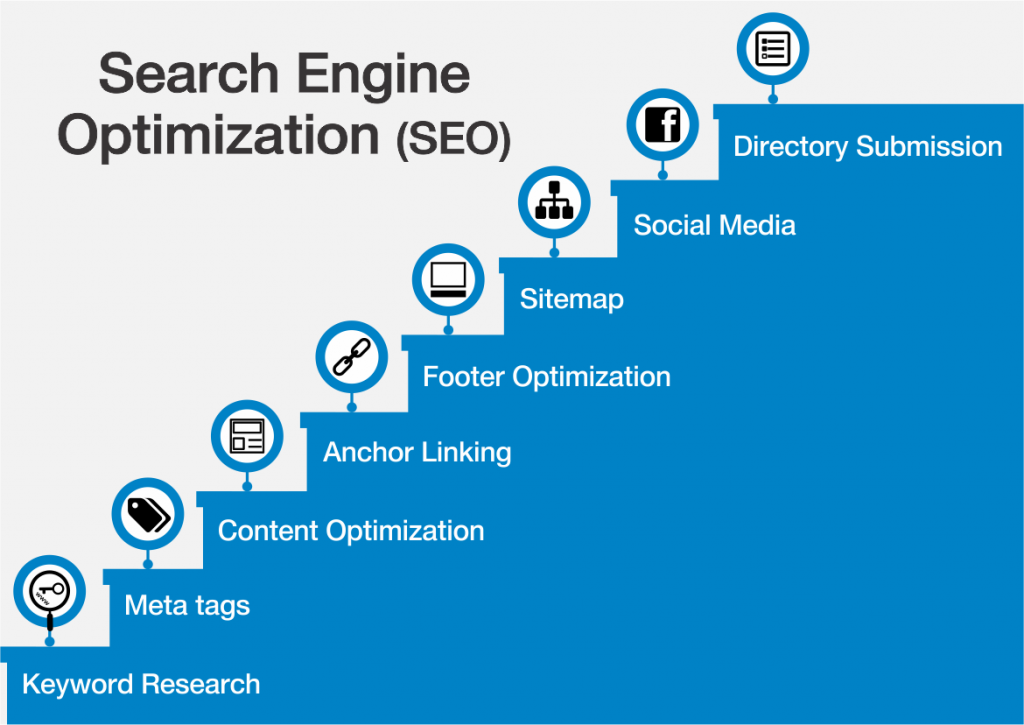
\includegraphics[scale = 0.2]{SEO.png} \end{center}
\vspace{0.5cm}
Le référencement naturel est l’art de positionner un site naturellement dans les premiers résultats des moteurs de recherche grâce à des mots clés, du contenus, ou des médias par exemple. Dans l'utilité d'un site internet c'est primordial car plus vous apparaissez haut dans les résultats de recherche, plus les utilisateurs vont cliquer sur votre lien au lieu de ceux des concurrents.
C'est donc la chose la plus importante pour un site internet.

L'équipe de référenceurs spécialisés en immobilier de La Boîte Immo doit s'adapter en permanence aux évolutions et mise à jour de google et doit remettre en forme le code des sites clients en fonction de leurs positions sur les moteurs de recherche et tout ça pour que ces sites restent attractif tout au long de la collaboration avec les clients.

Pour permettre aux référenceurs un suivi détaillé et en continu  des prestations fournis aux clients Google Analytics, Google Search Console ainsi que Google Tag Manager sont intégrés par défaut aux Back-Office de l'entreprise. De plus, tous les trois mois les clients peuvent demander un bilan complet à l'interlocuteur commercial.

\medbreak
\textbf{Référencement Adwords - SEA}

\vspace{0.5cm}

\begin{center} 
\includegraphics[scale = 0.7]{Adwords.png} \end{center}
\vspace{0.5cm}
Adwords est la régie publicitaire de Google qui permet de faire un complément au référencement naturel mais qui, contrairement à ce dernier,  est payant. Les annonceurs paient aux clics les annonces mises en avant en fonction de leur qualité et de leur pertinence. Plus l'annonce est pertinente plus le prix au clic est bas et inversement, il faut donc cibler des requêtes précises grâce à des mots clés.
En effet, Google Adwords permet de rendre un site beaucoup plus attractif et donc permet de faire venir plus de visiteurs car le réferenceur achète la position dans les résultats publicitaires de Google. Le classement des sites clients dans Google se fait donc en fonction du choix des mots clés et du montant du coût par clic, en ordre décroissant.

L'équipe de référenceurs à La Boîte immo est expérimentée, diplômée et certifiée Google. Elle participe tous les ans à des formations et conférences nationales / internationales.

L'équipe du pôle référencement effectue un suivi constant de toutes les prestations de tous les clients afin d'être toujours positionné sur la première page des principaux moteurs de recherche.

\newpage
\medbreak
\textbf{Référencement International}

Lorsqu'on parle de référencement on ne peut pas mettre de coté toute la partie internationale des utilisateurs surtout dans l'immobilier quand on voit leur place importante dans ce marché:

\vspace{0.5cm}
\begin{center} 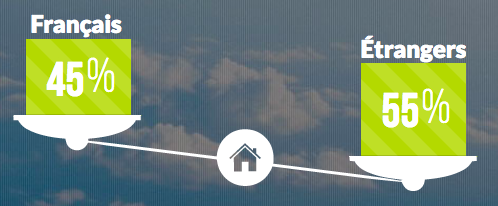
\includegraphics[scale = 0.5]{balance.png} \end{center}
\vspace{0.5cm}

Dans le monde 75\% des utilisateurs des moteurs de recherche ne consultent que la première page de résultats ce qui rend indispensable pour tout site de s'y positionner pour être le plus attractif possible sur le marché étranger afin d'attirer le plus de potentiels nouveaux clients ce qui est un atout considérable.

Un référencement bien pensé et bien utilisé permettra donc un bon positionnement du site sur les moteurs de recherche internationaux.

Après avoir conquis le marché français, La Boite Immo se lance dans la recherche de clients étrangers. Ainsi, après son développement au Luxembourg en janvier 2016 et son accord exclusif avec IPM Groupe Belgique en février 2017 les experts accompagnent les agences clientes pour déployer leurs campagnes sur les marchés anglais, espagnol, portugais, italien et allemand.

\vspace{0.5cm}

\begin{center} 
\includegraphics[scale = 0.4]{map_ref_international.jpg} \end{center}

\vspace{0.5cm}
\newpage
\subsection{Implantation}
\subsubsection{France}

La boite immo compte aujourd’hui plus de 100 salariés depuis juin 2018 avec une majorité présente dans le VAR à Hyères. Mais grâce a son envol fulgurant ces dernières années avec de multiples rachat d'entreprises, la société possède désormais des locaux un peu partout en France comme à Paris, Bordeaux, Montpellier, Lyon et Sophia Antipolis en plus de celui de Hyères qui va bientôt être déplacé dans de nouveaux locaux de 3000 m².
Ses commerciaux travaillent sur la France entière afin d'acquérir chaque jour de nouveaux clients.
\vspace{0.5cm}

\begin{center} 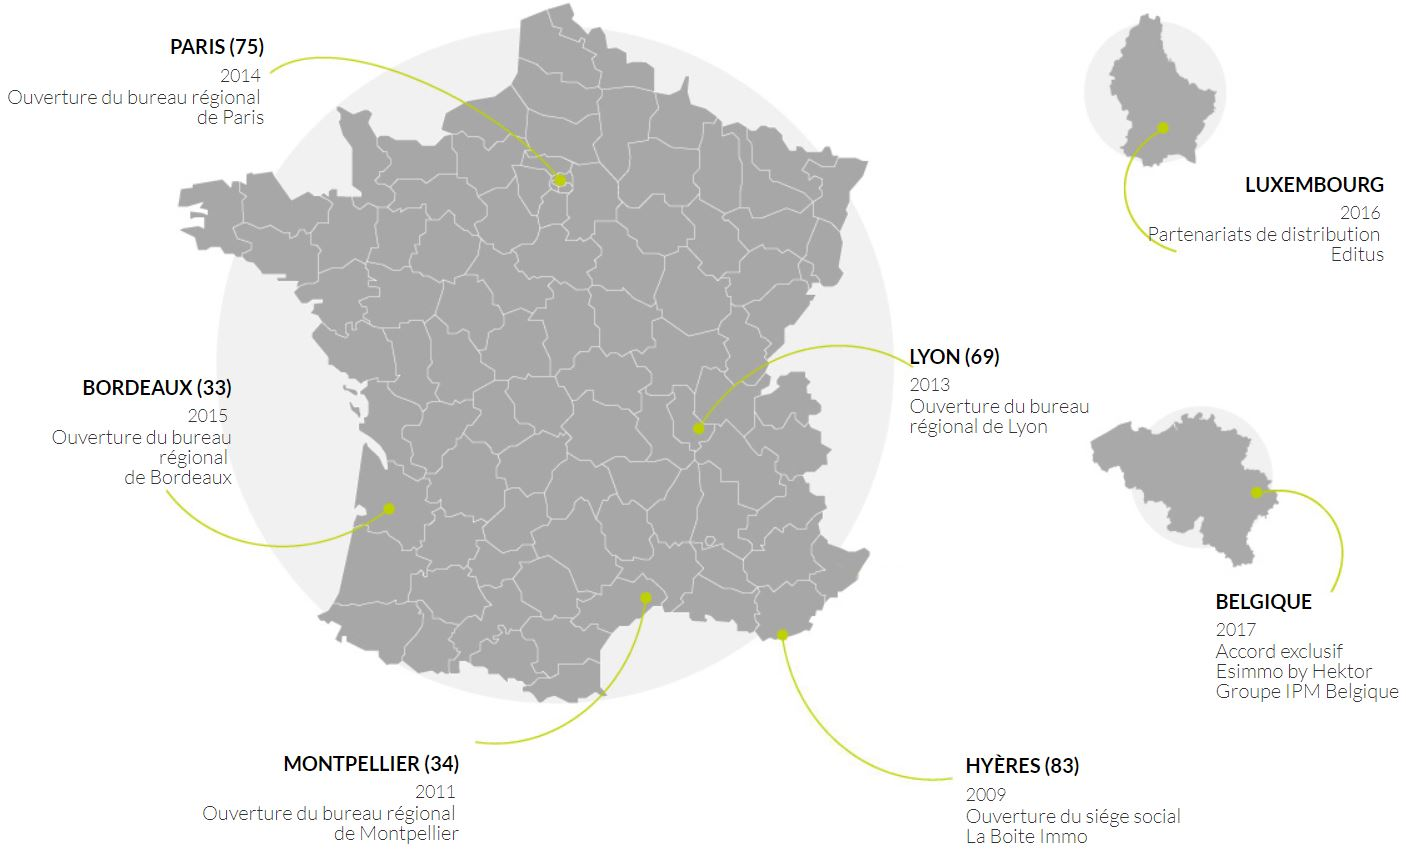
\includegraphics[scale = 0.4]{Map.JPG} \end{center}

\newpage

\subsubsection{International}

La société grandit de jours en jours et s'étend à l'étranger : Ouverture d'une agence commerciale au Luxembourg, partenariat en Belgique avec IPM Groupe, branche commerciale Prévisite aux USA, ouverture d'une agence de production technique en Tunisie (qui est une aide non négligeable pour arriver à satisfaire tous les clients). De plus La Boite Immo peut compter sur des revendeurs et revendeurs exclusifs partout dans le monde pour faire parler d'eux et elle ne compte pas s'arrêter là dans la conquête du monde de l'immobilier. 

\vspace{0.5cm}

\begin{center} 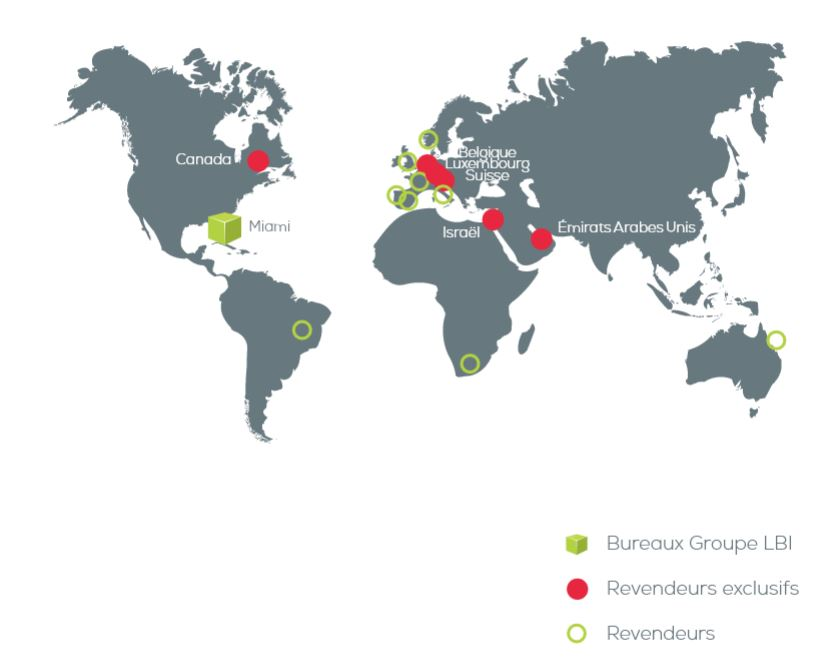
\includegraphics[scale = 0.7]{ImplantationMondiale.JPG} \end{center}

\newpage

\subsection{Données financières}
Comme La Boite Immo est devenu logiciel numéro 1 des agences immobilières indépendantes elle rachète petit à petit tous ses concurrents direct et fait croître son chiffre d'affaire de façon exponentielle avec un objectif quasiment chaque année atteint de 1 million de chiffre d'affaire en plus de l'année précédente.
\vspace{0.5cm}

\begin{center} 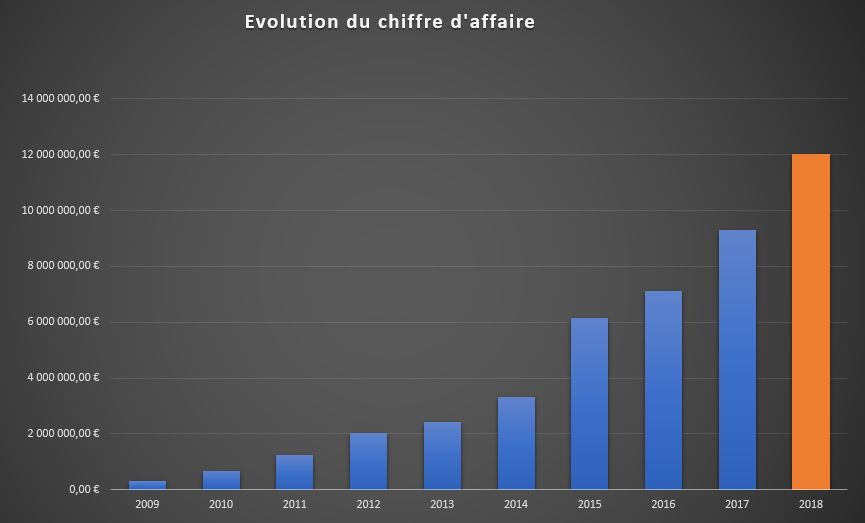
\includegraphics[scale = 0.5]{GraphCA.JPG} \end{center}

\vspace{0.5cm}
Malgré les objectifs déjà très ambitieux sur le chiffre d'affaire de la société  et déjà bien dépassé en 2017 avec +2 215 000€ et 9 320 000€ de chiffre d'affaire, elle a pour objectif de pulvériser les records avec plus de 12 000 000 d'euros pour l'année 2018 Ce qui semble plutôt en bonne voie pour l'instant.

\newpage

\section{Contexte du stage}
\subsection{Besoin de l'entreprise}

Gagnant de plus en plus en notoriété et en clients La Boite Immo voit de plus en plus de clients sensibilisé sur ce qu'est le référencement et surtout sur ce qu'est son utilité. Ainsi, Le pôle SEO, se voit vite en manque d'effectif pour continuer à être aussi efficace et se voit dans le besoin d'une mutualisation d'un maximum de taches de façon à faire en quelque clics ce qui leur prendrait plusieurs minutes en temps normal pour plus se concentrer sur l'optimisation de ces sites. 
Possédant déjà un outil pour les aider (l'outil Edouard), il manquait cruellement de fonctionnalités: Il ne pouvait pas être utilisé par d'autres personnes que les référenceurs eux même de part sa complexité ce qui rendait le suivi client au niveau du SEA / SEO pour les commerciaux plutôt complexe et demandait des intermédiaires avec les référenceurs ce qui leur rajoutait encore plus de travail.

\medbreak
\textbf{Fonctionnement global}

A La Boite Immo l'outil incontournable de gestion interne s'appelle Alfred. Il permet à l'entreprise de gérer tous les projets qu'elle a depuis un même outil autant au niveau commercial que référencement, gestion de projet intégration ou autres design SAV\footnote{Service après vente}.

Plusieurs étapes obligatoires précèdent la livraison du site web et/ou logiciel Hektor:

\begin{itemize}
\item Tout d'abord un commercial met en place un cahier des charges avec le client et le transmets au service comptable.
\end{itemize}
\begin{itemize}
\item Une fois validé, le dossier passe par un chef de projet.
\end{itemize}
\begin{itemize}
\item Ce dernier est crée dans l'outil Alfred une nouvelle fiche client.
\end{itemize}
\begin{itemize}
\item Une fois que le client est enregistré, il faut lui créer les onglets correspondant au contrat : site web et/ou Hektor.
\end{itemize}

\newpage

Une fois terminée, voici à quoi ressemble une fiche client :
\begin{center} 
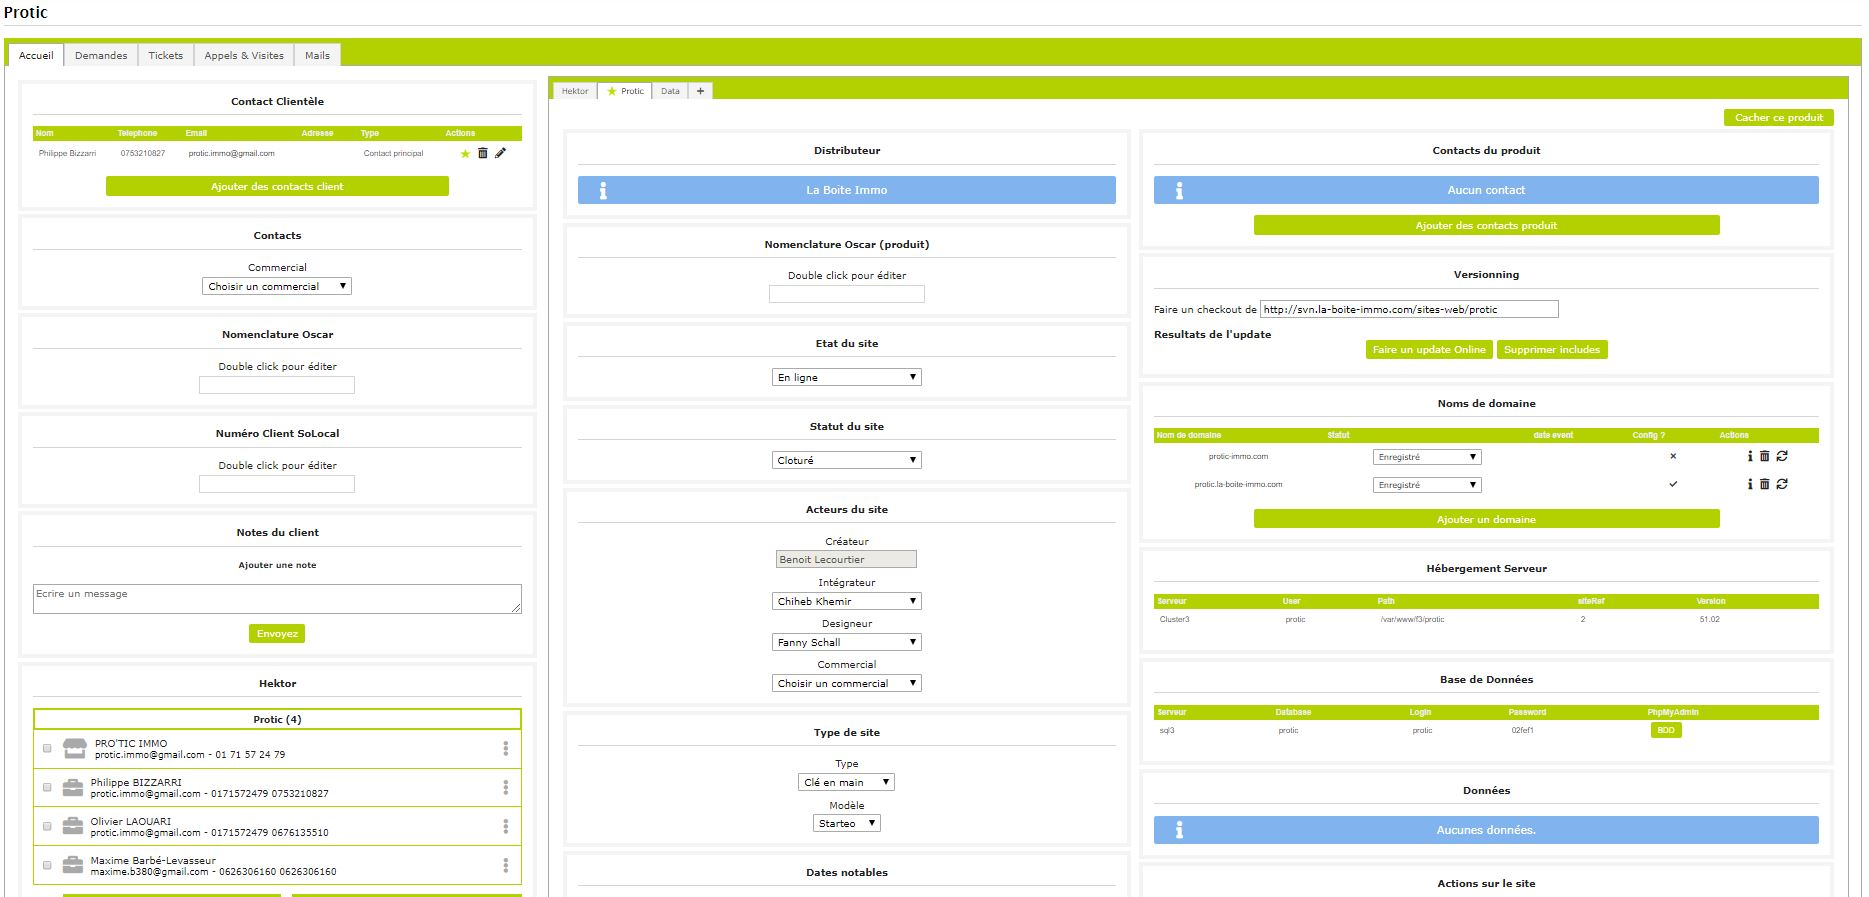
\includegraphics[scale = 0.3]{FicheClient1.JPG}
\end{center}

\vspace{0.5cm}

Ensuite le statut du site passe au statut : A Designer.

\begin{center} 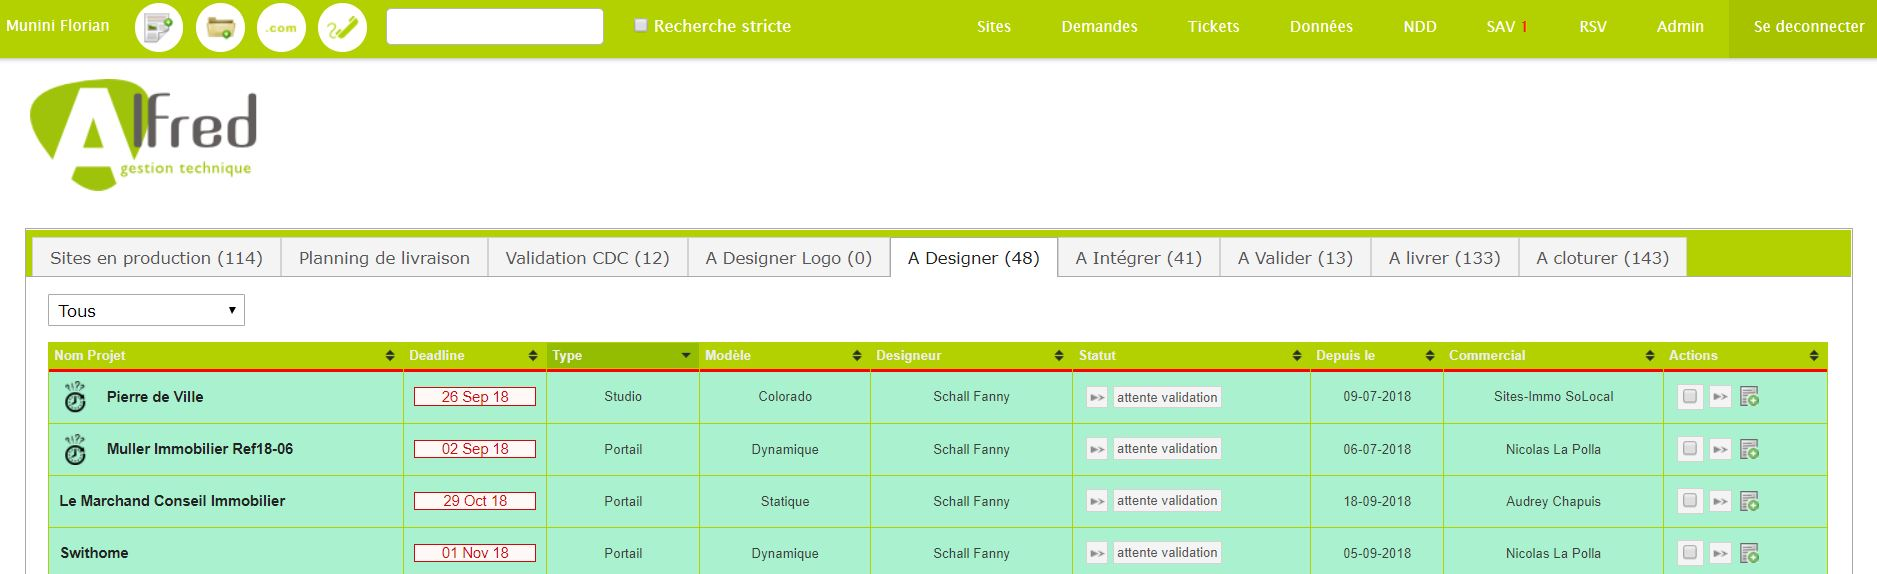
\includegraphics[scale = 0.3]{A_designer.JPG} \end{center}

Les designers piochent leur travail dans cette liste un site qui colle au planning en cours pour fournir une première maquette au client.
Une fois la maquette validée par le client le site passe en statut "A intégrer".

\vspace{0.3cm}

\begin{center} 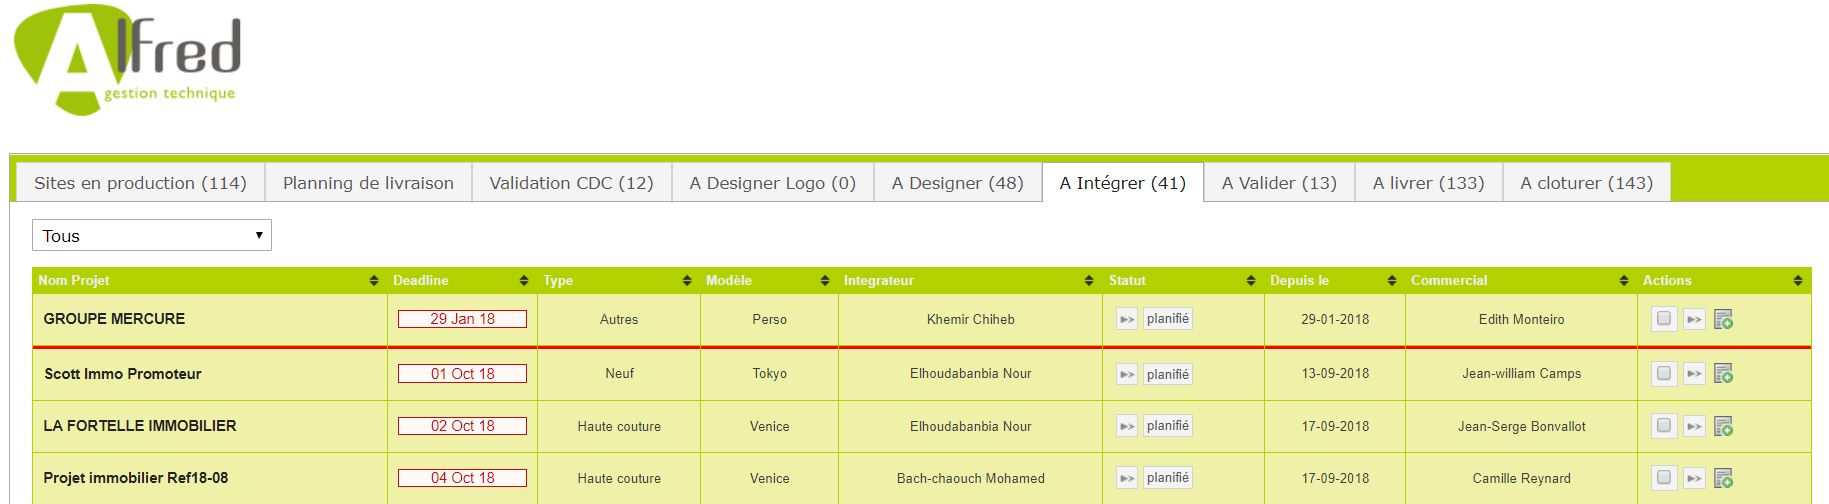
\includegraphics[scale = 0.3]{A_integrer.JPG} \end{center}

\newpage

Le chef de projet doit par la suite attribuer ce site à un intégrateur.\newline
Lors de la création d'une fiche client si Hektor est compris dans le contrat, une instance est automatiquement créée, du coup le client peut directement entrer ses biens, ses collaborateurs et toutes les autres données disponibles. \newline 
Pour des clients possédant un logiciel avant Hektor (plus ancien), une récupération de toutes les anciennes données est faites par les chefs de projets grâce à Hektor Import.

\vspace{0.5cm}

\begin{center} 
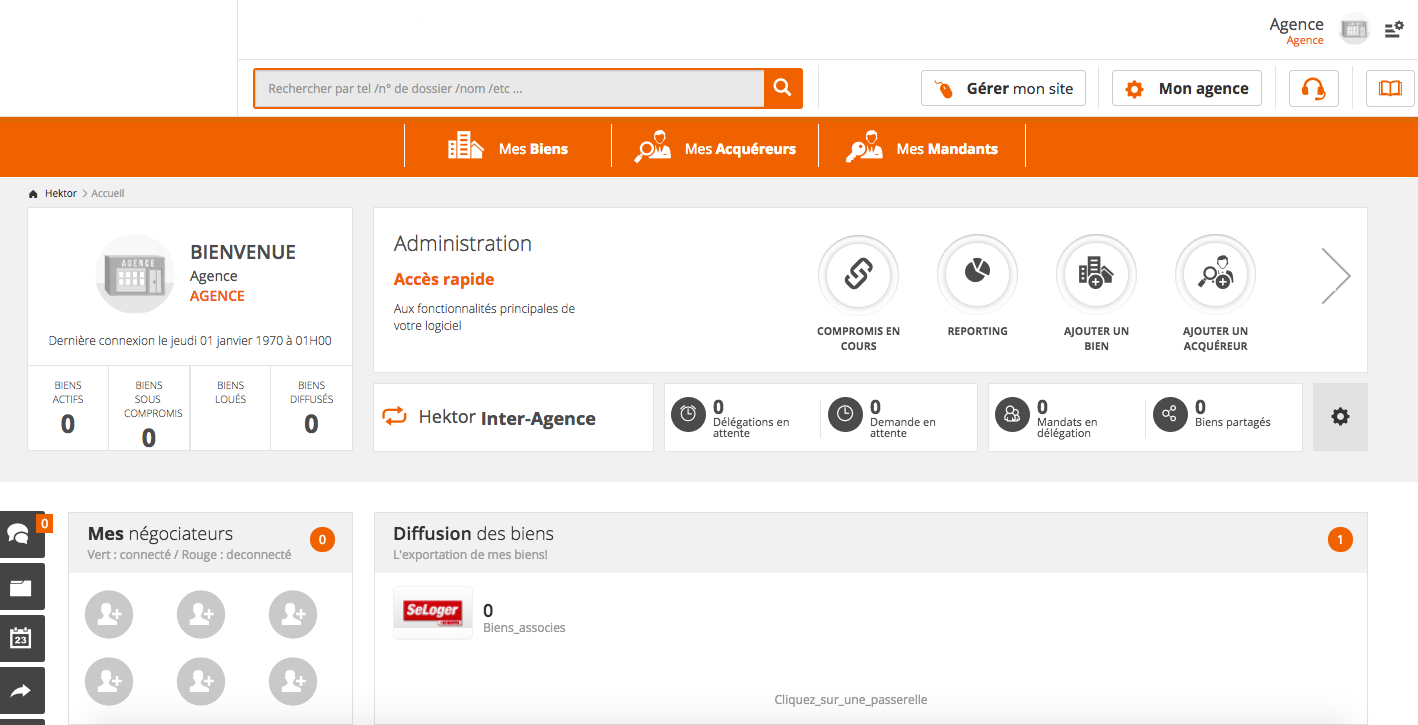
\includegraphics[scale = 0.4]{hektor_vide.png}\hfill
Profil Hektor
\end{center}
\vspace{0.5cm}

Dans un même temps, Jean Philippe LE GLEUHER, gérant du pôle référencement fait  une planification de livraison pour la prestation SEO sur les sites web. \newline
Il existe deux types de projet de site web : les sites avec et sans référencement. Même si un client choisi de ne pas prendre de prestation SEO, les référenceurs effectuent quand même certaines actions générique au cas où ils voudraient prendre une prestation de référencement comme par exemple la création d'un compte Google Analytics, la vérification des routes avec l'ajout de balise de référencement simpliste en prévision.
Pour qu'un référenceur effectue une prestation sur un site, il faut qu'avant toute chose l'intégrateur ait finis de développer le site.\newline
\newpage
Dans son ancienne méthode, Jean Philippe devait lui même éditer ses plannings et ceux des autres référenceurs. Ensuite il devait créer des fiches SEO et NO SEO pour les intégrateurs.

\begin{center}

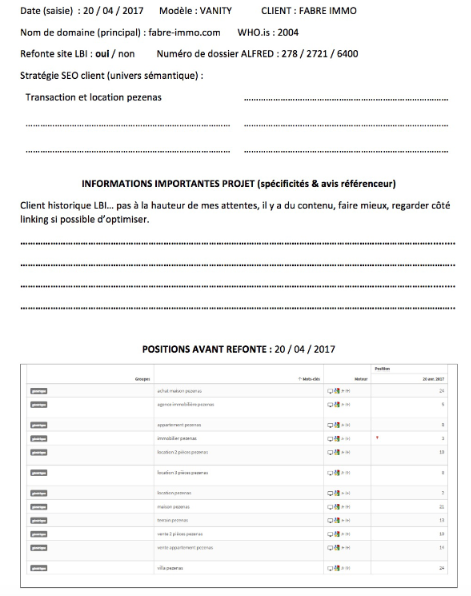
\includegraphics[width=7cm]{seo1.png}
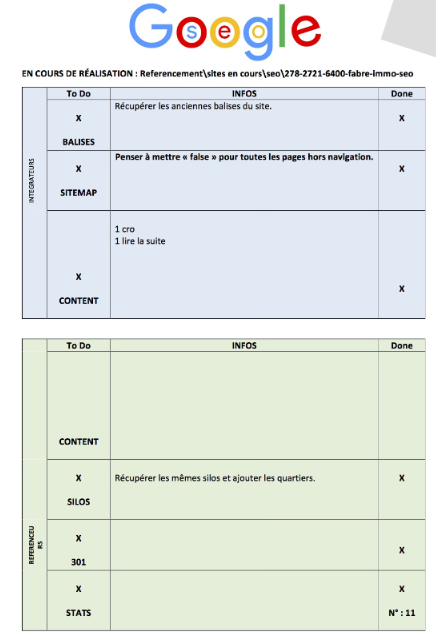
\includegraphics[width=7cm]{seo2.png}\hfill
Fiche SEO
\end{center}
\vspace{0.5cm}
Cette fiche était à la fois pour les intégrateurs et pour les référenceurs et elle était disponible dans un dossier dedié au projet sur le réseau Antonov de l'entreprise.

Une fois la prestation SEO faite, le site peut être livré au client par le commercial.

En plus de devoir effectuer des prestations SEO sur les sites, les référenceurs sont aussi chargés de repasser et d'entretenir tout au long de l'année pour tenir leurs engagements envers le client d'être toujours bien positionné.


\newpage
\subsection{Objectifs du stage}

L'objectif principal de ce stage était que pour les référenceurs de La Boîte Immo  les petites taches de quotidien sur l'outil Edouard, qui sont extrêmement chronophage et répétitives avec un panel de clients aussi grand, soient le plus simple, rapide et automatisé possible et leurs donnent le moins d'actions à faire. Ensuite il fallait aussi optimiser, dynamiser et améliorer beaucoup d'autres fonctionnalités qui, avec les rachats de nouveaux parcs clients extérieur et l'évolution de pas mal d'outils, engendraient beaucoup de problèmes. Par ailleurs il y avait une longue liste de rajout de nouvelles fonctionnalités que les référenceurs avaient pensé de part leur utilisation quotidienne de l'outil. De plus Jean Philippe LE GLEUHER ainsi que Arnaud WEBER avaient pour idée de mettre des fonctionnalités spécifiques pour des intervenants sur le site qui ne sont pas des reférenceurs comme par exemple la génération automatique de rapport SEA/SEO, pour que les commerciaux puissent d'eux même l'utiliser et le montrer aux clients, à l'intérieur duquel une longue liste de statistiques, de données et de graphiques seront présent\\
Enfin d'autres objectifs ressortent. Je devais tout d'abord apprendre comment le référencement était fait à La Boite Immo car il est très fourni et complexe, apprendre comment fonctionne chaque outil de référencement SEO/SEA pour savoir ce qui était pertinent à afficher sur Edouard et comment utiliser les différentes API, Ensuite être capable de mettre en place mettre en place des prestations de référencement sur des sites clients tout en comprenant leur fonctionnement.

\newpage
\subsection{Contexte technologique}
\subsubsection{Bobcat, le framework 100\% La Boîte Immo}
Bobcat est un framework privé développé en PHP et crée par le Lead Developer du pôle Recherche et Développement Jonathan KOWALSKI en juillet 2013 et qui, à ce jour continu d'être implémenté et mis a jour par les développeurs du pôle R\&D. C'est le cerveau de tous les sites et de la plupart des outils internes de La Boîte Immo :
Edouard, Modèles de sites, Espace client, Auditor, Gérer mon site, Tâches en console utilisé par le Cron\footnote{Cron est un programme qui permet aux utilisateurs des systèmes Unix d’exécuter automatiquement des scripts, des commandes ou des logiciels à une date et une heure spécifiées à l’avance, ou selon un cycle défini à l’avance.} du serveur.
Il est donc composé de plusieurs répertoires : Applications, Sites, Console, Controller, Models.

Le répertoire Application contient des sous-répertoires avec le code du back-end des différents outils internes ou externes.\\
Le répertoire Sites contient tous les modèles des sites. Ce qui correspond à toute la panoplie des versions de site web proposé par La Boite Immo à ses clients.\\
Console contient toutes les tâches utilisées dans le Cron du serveur.\\
Controller contient tous les controllers \footnote{Couche du modèle MVC : Model View Controler.Ce sont comme des "managers" qui ont pour mission que toutes les ressources souhaitées pour accomplir une tâche soient déléguées aux travailleurs corrects.} 
génériques utilisés par chacun des autres sous-répertoires qui gèrent les requêtes des utilisateurs. Ils sont responsable de retourner une réponse avec l’aide mutuelle des couches Model\footnote{Couche du modèle MVC qui contient les données à afficher} et Vue \footnote{Couche du modèle MVC qui contient la présentation de l'interface graphique}.
Models est le répertoire où tous les templates\footnote{Les templates représentent la couche Models du modèle MVC} de chaque applications ou modèles de sites sont définis.

\textit{Pour des raisons de confidentialité et de propriété intellectuelle, l'architecture visuelle (par screenshoot ou par schéma) ne pourra être fournie.}

\newpage

\subsubsection{Autres technologies utilisées}
\begin{itemize}
\item \textbf{PHP :} Officiellement: Hypertext Preprocessor est un langage spécialement conçu pour le développement d'applications web. Il permet de la rendre dynamique en permettant de discuter avec une base de données et il s'intègre facilement au HTML tout en étant orienté objet. C'est le langage principal de tous les controllers de Bobcat.
\item \textbf{Javascript :} Le Javascript est aussi un langage de programmation orienté objet. Dans le cas de Bobcat il est utilisé en combinaison avec le PHP et il permet de rendre des pages web interactives assez facilement en jouant/modifiant le HTML de manière asynchrone\footnote{Qui n'interfère pas avec ce qui se passe sur la page courante durant son exécution}. Je l'ai utilisé pratiquement dans toutes mes pages HTML pour les animations et surtout pour les appels Ajax. Un appel Ajax permet de questionner un controller et récupérer le résultat d'une requête dynamique sans rafraîchir une page.
\item \textbf{SQL :} Le SQL ou Structured Query Language SQL est un langage de base de données relationnelle. Il permet de créer des bases et des tables, ajouter, mettre à jour, supprimer des données de ces tables\footnote{Ensemble de données organisées sous forme d'un tableau où les colonnes correspondent à des catégories d'information}. Je l'ai utilisé dans mes controllers PHP afin de questionner la base de données.
\item \textbf{Smarty :} Smarty est un framework\footnote{Sur couche d'un langage existant dans le but de faciliter une de ses utilité} et plus précisément un moteur de template pour PHP. Il facilite la séparation entre la logique applicative et la présentation visuelle. Il permet de séparer complètement le HTML et le PHP (ne pas avoir des balises php en plein milieu du HTML) et de ne pas avoir des duplications de code HTML. 
\item \textbf{Less :} Less est un langage dynamique de génération de CSS. Son utilité était surtout pour déclarer des variables CSS ce qui permettait de les réutiliser à plusieurs endroits pour éviter la duplication de code. Exemple une taille générique à plusieurs classe CSS ou encore la couleur principale d'une page.
\item \textbf{Bootstrap :} Bootstrap est une compilation d'outils d'aide à la création du design (graphisme, animation et interactions avec la page dans le navigateur ... ) de sites et d'applications web. C'est donc un framework, une librairie de classe CSS avec des designs pré-définis. Étant responsive\footnote{Appellation donnée à un site web pour dire qu'il s'adapte à tout type de support (téléphone,tablette,pc,..) en étant toujours facielement consultable}, il m'a m'a été très utile pour rendre ce que j'ai développer multi-plateforme.
\end{itemize}

\newpage

\section{Les projets du stage}
\subsection{Familiarisation avec les services}

\subsubsection{Référencement}

Ayant comme projet de stage le développement et l'amélioration de l'outil Edouard, qui est l'outil indispensable de toute l'équipe de référenceur de La Boite Immo, j'ai dû tout naturellement me plonger dans le référencement et plus particulièrement dans la façon de faire d'en faire à La Boite Immo. C'est pourquoi j'ai, dès les premier jours, été formé sur toute cette partie ce qui m'a fait toucher en même temps à pleins de domaine. Premièrement j'ai pu voir toute la partie intégration des sites qui est en étroite collaboration avec la partie SEO car avant de mettre en ligne un site il faut que son wording\footnote{tous les textes mis en avant sur le site} soit en accord avec ce que propose le site pour être référencé sur le thème qui les intéresse le plus: il faut donc donner du poids aux mots\footnote{Par exemple en HTML avec des balises qui permettent de mettre en gras le mot va plus facilement être référencé qu'un mot qui est écris normalement}. De la même façon il faut que toute la face caché du site (que l'on ne voit pas forcément en visitant le site) c'est à dire les description des pages, les balises titres, les routes vers les pages ou encore les description caché des images qui vont quand même être pris en compte par google, soient aussi en accord avec les ce que recherche à faire le site. C'est donc un travail minutieux et qui doit être bien guidé avec des façons de faire à respecter pour permettre une gestion de masse des sites bien plus simple. Deuxièmement j'ai dû me familiariser avec tous les outils de référencement utilisé par La Boite Immo car dans la procédure qu'ils utilisent en SEO chaque nouveaux clients (Qu'il ai choisit une prestation de référencement ou non) se doit d'avoir un compte Google Analytics qui est un compte de suivi de toutes les statistiques lié au SEO pour que, même si le client n'a pas de prestation de référencement, si plus tard il en veut une, il aura toujours des données des mois passés. C'est un outil complexe à comprendre quand on ne possède que des base en SEO car il regorge de fonctionnalités et comme c'est l'outil principal qu'utilise La Boite Immo pour ses prestations ce fut un gros travail d'adaptation. Ensuite chaque nouveaux clients se voient aussi attribuer un compte Google Search console pour le suivi d'indexation / position sur les résultats des moteurs de recherche et pour les erreur webmaster\footnote{Regroupe toutes les erreurs type 404 not found sur une page, les erreurs serveurs,...}. Enfin, uniquement pour les clients ayant choisis une prestation de référencement un compte MyPoseo leur est crée: c'est un compte payant (où il faut payer par requêtes par mots clés le tout par jour) qui permet de remonter des informations bien plus précises que sur les autres outils et d'autres qui ne sont disponibles que sur cet outil.

\newpage

\subsubsection{Recherche \& Développement}

Juste après avoir finis de me former sur les outils de référencement est arrivé le début du développement de Edouard. C'est à ce moment là que j'ai commencé à vraiment attaquer au code et donc que j'ai commencé a apprendre à utiliser Bobcat. Grâce à plusieurs projets personnel en Symfony\footnote{Est aussi un framework PHP mais celui ci n'est pas privé} utilisant approximativement le même univers de développement je me suis plutôt vite adapté aux bases de son utilisation et de son installation. Par la suite, grâce à l'aide précieuse du Lead Developer Jonathan KOWALSKI, j'ai commencé par rajouter des petites fonctionnalités pour me familiariser avec l'outil et avec toutes les options qu'il propose. Étant motivé je me suis attardé sur chacune des fonctions principales d'Edouard pour que j'ai au plus vite une vue d'ensemble de ce qu'il contient ainsi que du potentiel temps que je devrai passer dessus si jamais j'avais à modifier une de ces dernières.J'ai pris plusieurs fois peur de la taille de l'arborescence de certaines parties car, étant privé, le framework ne possède quasiment aucune documentation et donc j'avais absolument besoin de Jonathan pour répondre à mes questions et il a été extrêmement présent à ce sujet et m'a vraiment souvent renseigné pour m'aider. C'est donc après plusieurs semaines de découverte, avec un développement un peu ralenti à cause de ça, que je me suis senti vraiment à l'aise avec l'outil et que j'ai attaqué vraiment les grosses fonctionnalités.

\newpage
\subsection{Edouard, l'outil interne des référenceurs}
\subsubsection{Présentation}
Edouard est un outil de gestion de mesure et d’analyse de toutes les campagnes de référencement naturel et payant des clients de La Boite Immo.Cet outil a été développé pour permettre à l'équipe de reférenceurs d'avoir une vue autant d'ensemble que client par client du retour de tous les outils utilisé pour le référencement.Cet outil leurs est donc indispensable étant donné leur parc de clients conséquent. Les données sont disponibles pour un projet client mais aussi agrégées par modèle, gamme de site et site référence. De plus cet outil permet aussi d'avoir un suivis des actions faites sur chaque clients par les référenceurs et de le trier dans différentes catégories selon son statut (en audit, en optimisation, en livraison, livré ou encore si ce sont des clients SEO ou non). Une autre des fonctionnalités de cet outil est toute la partie documentation. Il dispose d'une partie blog où toutes les bases du SEO, que ce soit pour comprendre les graphiques ou comment marche le SEO, sont expliqués ainsi qu'un récapitulatif de toutes les procédures générique du pôle et des mises à jour Google où sont cités tous les impacts qu'elles ont eus sur les prestations des clients. Enfin cet outil permet d'avoir des fiches clients, modèle, gamme de site et site référence qui regroupent toutes les données des outils de référencement. On peut y voir tout type de graphiques de regroupement de données, que ce soit des graphiques venant de Google Search Console, Google Analytics ou encore MyPoseo ainsi que des chiffres précis sur les statistique SEO et SEA.  \\

\newpage
\subsubsection{Gestion de projet}

Pour cette partie, ayant M. Le Gleuher comme client direct j'ai dû travailler en étroite collaboration avec lui et, par chance, comme nous nous entendions très bien nous avons pu nous mettre d'accord pour effectuer fonctionnalité par fonctionnalité selon les besoins qu'il avait et les idées qui lui venaient avec validation du code avant mise en ligne par le lead developpeur M. Kowalski. Nous avons donc choisi la méthode Agile comme modèle de gestion de projet couplé à un Trello très actif en l'adaptant aux conditions et besoins de La Boîte Immo. C'est donc sans aucun accrochage que le projet s'est déroulé. De plus M. Le Gleuher était extrêmement à l'écoute de mon retour sur les différentes idées qu'il avait car comme il n'avait pas la vision d'un développeur il s'en remettait à moi pour réajuster les tâches afin que ça paraisse faisable car il fallait pouvoir vite enchaîner sur d'autres fonctionnalités et inversement quand je trouvais une façon plus simple ou plus optimisé de faire une des fonctions je le tenais de suite au courant pour valider ce changement dans la finalité de la tache. 

\vspace{1cm}

\begin{center} 
\includegraphics[scale = 0.7]{processusProjet.jpg} \end{center}
\vspace{1cm}
\newpage

\subsubsection{Les missions}

\begin{itemize}
\item \textbf{Changement de toute la librairie des graphiques des fiches clients}		
\end{itemize}
	 	Les anciennes fiches clients ne possédaient que quelques graphiques GoogleChart\footnote{Librairie de graphiques de Google} de données qui n'étaient pas modulable, non  responsive et avaient un design qui ne faisait pas du tout moderne:

\begin{center}
 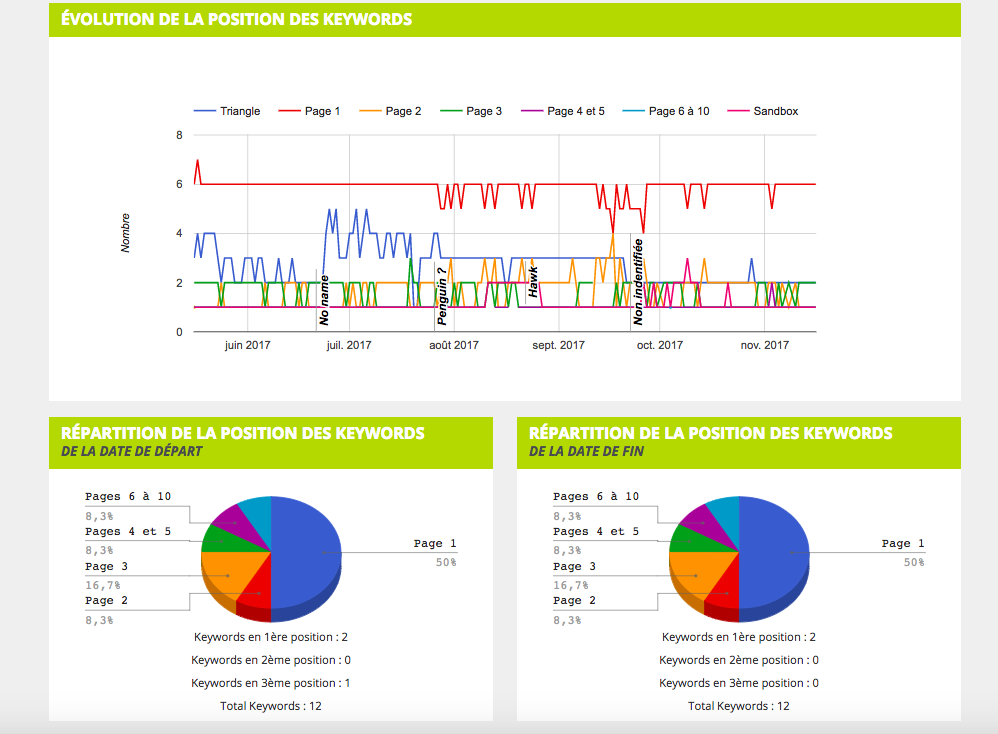
\includegraphics[width = 15cm]{projetData2.png}
    \textit{Page Projet avec les anciens graphiques}
\end{center}
		
        C'est donc fin juin que j'ai commencé à m'attaquer à la migration de la librairie Google Chart vers la librairie HighCharts\footnote{Librairie de graphiques générique} qui est une librairie payante mais qui possède bien plus de fonctionnalités. J'ai dû pour ce faire m'entretenir longuement avec le développeur du pôle Hektor Romain Valy  ainsi que son Lead Developpeur Jules Renard pour qu'ils m'expliquent les controllers qu'ils avaient déjà fait pour faciliter son utilisation car c'est la librairie principale utilisé sur les outils en relations avec Hektor. 
        Après cette formation je suis rentré dans le vive du sujet et j'ai changé un par un les graphique ce qui n'était pas simple car tout était formaté pour générer des GoogleChart qui ont une syntaxe très particulière j'ai dû donc toucher à des controllers très loin dans l'arborescence pour changer toute la façon de renvoyer les données et la rendre plus générique. J'ai tout de même gardé à certains endroits la possibilité de changer dynamiquement de  GoogleChart vers HighCharts et inversement, car dans la nouvelle librairie qui m'a été fournit il n'y avait pas la possibilité de mettre des annotations sur les graphiques ce qui était quelque chose qui, pour le pôle référencement, était très important pour placer des notes sur les mises à jour de Google pour voir les impact que ça avait sur les prestations des clients.
        
\begin{itemize}
\item \textbf{Migration vers une version plus récente de l'API de Google Analytics}
\end{itemize}
Après avoir fait le changement de la librairie graphique pour passer en Highchats, j'ai eu une grosse réunion avec  M. Le Gleuher pour que l'on discute des données qui étaient les plus pertinente à afficher sur les fiches clients Edouard car il manquait des données extrêmement importante. De plus le code de récupération déjà en place était fait au cas par cas et n'était pas modulable ce qui faisait perdre beaucoup de temps pour récuperer de nouvelles données. En étudiant l'API Google Analytics utilisé je me suis rendu compte que la version utilisé était considéré comme déprécié\footnote{Situation où une ancienne fonctionnalité est considérée comme obsolète au regard d'un nouveau standard} donc comme je devais rajouter des données et rendre le code modulable dans tous les cas ce qui allait me faire changer une grosse partie du code j'ai demandé l'accord du  lead developpeur M. Kowalski pour savoir si je pouvais changer directement l'API Google Analytics. Il a accepté mais comme l'API était utilisé sur plusieurs autres outils interne il m'a dit que je devrai aussi me plonger dans le code de chacun d'eux pour tester, et changer si il faut, le code de ces derniers pour qu'ils continuent à marcher. Après avoir étudier la question j'ai accepté en sachant qu'il allait y avoir énormément de code  à toucher sans trop savoir les répercussions que ça allait avoir. Nous avons donc décidé avec M. Kowalski que la façon la plus simple de faire serait de réussir à changer toute l'API mais avoir en retour final toujours la même arborescence et forme de code qu'il y avait avec l'ancienne version pour que tous les outils qui l'utilise n'aient rien à changer dans leur code. Je suis donc parti sur cette optique la en rendant en plus la possibilité d'avoir un code modulable pour gagner le plus de temps possible en cas de rajout de nouvelles données.Après avoir réussi la migration j'ai donc dû aller tester dans l'outil Gérer mon site, qui permet aux clients de La Boite Immo de changer quelques éléments sur leur site web sans passer par les développeurs comme par exemple certains textes ou certaines images, et qui permet aussi de regarder un bref résumé de quelques données de référencement de leur site. Après quelques jours de débug sur GMS\footnote{Gérer mon site} j'ai pu tout mettre en ligne.

\newpage

\begin{itemize}
\item \textbf{Ajout de l'API Google Search Console et des données de Google Tag Manager}
\end{itemize}

Comme dit précédemment Edouard manquait déjà de données extrêmement importantes de Google Analytics mais en plus il ne possédait tout simplement pas de façon de récupérer des données de Google Tag Manager et Google Search Console qui sont des outils présents sur chacun des clients de La Boite Immo ce qui en faisait un problème plutôt urgent. Après m'être renseigné j'ai pu voir que les données de Google Tag Manager étaient accessible depuis l'API de Google Analytics d'une manière très similaire alors que par contre pour Google Search Console c'était toute une autre histoire car la façon d'utiliser l'API était bien différente et m'a posé aussi beaucoup de problèmes de droits de compte. En effet comme les comptes Google Analytics, Google Tag Manager et Google Search Console peuvent être lié, ils sont accessibles depuis la même API mais là où leurs utilisations différent c'est au niveau de la structure des requête car pour Google Analytics et pour Google Tag Manager la structure :est quasi identique: \newline \newline
- Il faut choisir une date de début et une date de fin pour savoir la période sur laquelle on veut les données. \newline
- Il faut choisir un ou plusieurs métrics qui seront les statistiques quantitatives du retour des requêtes. C'est à dire à quoi correspondent les chiffres (exemple si on prend Pages/session les retours correspondront au nombre moyen de pages vues par utilisateur).\newline
- Il faut choisir une ou plusieurs dimensions qui seront les attributs des métrics c'est à dire en fonction de quoi les données sont traitées (exemple si on prend en métric session qui correspond à la visite d'un utilisateur, et que on prend en dimension ville le résultat sera le nombre de visites d'un utilisateur par ville).\newline
- Il y a aussi la possibilité d'ajouter différents types d'options supplémentaires comme les filtres (exemple si on filtre les villes pour avoir uniquement celles qui commencent par la lettre "M" ce qui laisse une étendu très grande de possibilités),l'ordre d'affichage (exemple par date croissante) ou encore le nombre maximum de résultats qui m'a beaucoup servis pour optimiser le temps de chargement de la page fiche client vu le nombre conséquents de données récupéré en même temps.\newline \newline
Par ailleurs même si la structure de Google Search Console ressemble aux 2 autres outils sur la forme sur le fond les appels étaient totalement différents ce qui m'a fait redévelopper de tous nouveaux controllers, toujours de manière dynamique, que j'ai dû intégrer au reste des outils. Cette structure se définit de cette avec une période de temps et uniquement un choix très limité de dimensions sans avoir de metrics ni de filtres. On ne pouvait donc que ajouter à la requête certaines options limitées comme l'ordre d'affichage ou le nombre maximum de résultats le tout appelé d'une façon totalement différente que les deux autres outils. En arrivant à la phase de test de l'outil Google Search Console, des problèmes de permissions sont survenus et après plusieurs jours de recherche sur une documentation très peu fournis pour le langage PHP j'ai trouvé une solution qui fut une très mauvaise nouvelle pour le pôle SEO car il fallait, pour intégrer cette API passer un à un sur chacun des clients ayant un compte Google Search Console (soit quasiment tous) afin de donner une autorisation supplémentaire pour accéder aux données depuis l'API. Nous nous sommes donc mis tout le pôle référencement sur cette tâche qui nous a pris plusieurs jours.

\begin{itemize}
\item \textbf{Création automatisé d'un rapport pdf complet sur le SEO }
\end{itemize}
L'une des tâches les plus longues et importante fut sans aucun doute celle ci car c'était le but final de mon stage. Dès le début du mois de juin M. Le Gleuher m'a fait savoir que les commerciaux ne peuvent pas, sans son intervention au préalable au cas par cas, parler de où en est le référencement de leur site et comment il évolue car il faut automatiquement l'intervention d'un professionnel dans ce milieu pour ressortir les informations importantes ce qui posait un gros problème car le référencement intéresse beaucoup les clients. \newline
Pour réaliser cette tache je fus en constante collaboration avec le designer de La Boite Immo Guillaume Tedeschi qui m'a fait très rapidement le modèle graphique du futur rapport SEO de 23 pages. 
Par ailleurs en ce qui concerne sa création j'ai dû utiliser un outil développé pour PHP qui est Html2Pdf\footnote{Outil permettant de convertir de l'HTML (qui est simple à designer et qui donne pas mal de liberté) directement au format PDF qui lui est bien moins permissif et qui est compliqué à écrire en PHP} pour rendre sa création et son design bien plus simple car le pdf est très long et possède une charte graphique complexe. Après avoir intégré cet outil au Framework Bobcat j'ai commencé a faire le liens entre les données de la fiche client et le HTML de la base du rapport. Quand cela était fait il ne me restait plus qu'à réutiliser les données déjà présentes sur la fiche clients qui devait être aussi présente sur le rapport (ce n'était pas le cas de toutes) et surtout de rajouter les nouvelles demandé. Pour savoir quelles étaient les nouvelles données nous avons fait une réunion avec M. Le Gleuher pour qu'il me dise exactement où les trouver sur Google Analytics, Google Tag Manager ainsi que Google Search Console pour ne pas perdre de temps à chercher. J'ai donc commencé par 
 migrer l'API Google Analytics vers une version plus récente pour repartir sur de bonne bases non dépréciées et j'ai rendu toute cette nouvelle façon de récupérer les données dynamique car avant c'était du cas par cas (comme expliqué dans ma deuxième mission). Ensuite j'ai récupéré les données de Google Analytics qu'il restait à avoir sur le rapport ce qui fut une tache très répétitive car, ayant tout dynamisé, d'une donnée à une autre seul quelques paramètres changeaient. Après avoir tout récupéré de Google Analytics, je me suis attaqué au design total du rapport ce qui fut très très long car, certes c'est une page HTML mais comme ce sont des éléments fixe sur une feuille de papier tout se code en millimètres (car les imbrications entre les blocs sont très mal pris en compte lorsqu'on code en pixel pour le pdf) et surtout pour tester une quelconque ligne de code changer il fallait repasser par la génération du pdf qui est un processus qui devient très vite long plus on y rajoute du contenu. J'ai donc d'abord designer en entier la forme du pdf sans les données grâce aux ressources graphiques du designer puis j'y ai rajouter les données de Google Analytics. Enfin pour rajouter les dernières données venant de Google Tag Manager et Google Search Console j'ai eu beaucoup plus de mal comme je l'ai expliqué dans ma troisième mission. Après avoir tout récupéré les données demandé je suis passé à l'intégration au rapport et la s'est posé un autre problème: La génération du pdf était bien trop longue. Pour régler ce problème j'ai du donc réduire toutes les images a leur taille exacte de leur utilisation sur le rapport pour gagner de précieuses secondes (voir même minutes) ce qui pour finir en arrive à une génération dynamique, certes encore longue, mais avec un temps bien plus convenable car cela reste quand même un pdf de 23 pages avec un design fourni et énormément de données transféré.

\begin{itemize}
\item \textbf{Mensualisation de la récupération des données Majestic SEO}\footnote{Outil qui cartographie les liens entre les pages web, plutôt que le contenu du web en lui-même ce qui permet de voir à quel point les liens vers le site voulu sont pertinents}
\end{itemize}
L'équipe de référenceur de La Boite Immo propose à ses clients de prendre ou non une prestation SEO et ce qui change entre les deux est que si ils en prennent une ils ont, en plus du compte Google Analytics, Google Tag Manager et Google Search Console, un compte Myposeo qui est aussi un outil de statistiques SEO mais celui ci est payant par mots clés et par requêtes par mots clés mais est beaucoup plus précis tout en donnant accès à de nouvelles données qui ne sont disponible nulle part ailleurs. De plus il est possible de lier un compte Myposeo avec un compte Majestic SEO ce qui a donné l'idée à la dernière arrivante en août au pôle SEO pour seconder M. Le Gleuher: Caroline CASTRO, de rajouter ces données à la fiche client sans l'intégrer dans le rapport pour ne permettre que seul l'équipe de référenceurs y ait accès. Par ailleurs comme les données Myposeo sont les seules données stocké en base de données de manière quotidienne et automatisé (toutes celles de Google Analytics, Search Console et Tag Manager sont récupérées à la volée par des requêtes web) et que la récupération quotidienne des données Majestic SEO n'était pas très utile j'ai dû créer une nouvelle tache pour le Cron du serveur pour tout soit récupéré mensuellement.

\section{Apports du stage}
\subsubsection{Difficultés rencontrées}
Durant ce stage je n'ai pas rencontré beaucoup de difficultés à part deux qui m'ont pris beaucoup de temps.
La première fut l'absence de documentation sur le framework Bobcat puisqu'il est privé et uniquement pour La Boite Immo. Au début ce fut un gros frein pour l'avancement du code car M. Kowalski était souvent occupé et je ne pouvais pas lui poser de questions pour qu'il m'aide. J'ai dû donc plusieurs fois chercher à l'aveugle pour pouvoir avancer ce qui m'a fait perdre pas mal de temps.\newline
La deuxième fut, comme je l'ai cité précédemment, un problème lié à l'API Google Search Console et plus particulièrement à ses droits utilisateurs car le parc client de La Boite Immo est géré d'une façon bien spécifique et comme cette API n'est pas très bien renseigné, les informations sur ce cas particulier furent difficiles à trouver et après avoir trouvé une première solution je me suis rendu compte que pour l'appliquer partout il fallait faire des changements sur chacun des 6500 clients de La Boite Immo un après l'autre à la main. Donc pour éviter ça j'ai essayé de trouver une deuxième solution et j'ai, là aussi, perdu beaucoup de temps à chercher mais en vain ce qui donc a fait conclure à M. Le Gleuher que nous allions rester sur la première solution.

\subsubsection{Techniques}
D'un point de vue technique, ce stage m'a permis de continuer à m'améliorer en PHP qui est un langage que j'apprécie beaucoup et avec lequel j'avais déjà travailler plusieurs fois sur des projets personnels et scolaires. Il m'a aussi permis de m'améliorer énormément en Javascript qui était un langage que je n'aimais pas du tout avant et que maintenant j'adore et qui m'est très utile. Pour finir il m'a permis de m'améliorer en SQL car j'ai découvert des requêtes très complexe que je n'avais jamais vu avant.

De plus j'ai pu enrichir ma culture informatique en découvrant et travaillant sur de nouveaux concepts et mécanismes qui sont le Less, le Smarty et enfin le Cron.

Enfin, j'ai pu mûrir sur ma méthodologie de travail en approfondissant des domaines déjà abordés lors de ma formation : Programmation orientée objet, Gestion de Base de données mais aussi en apprenant des nouveaux paradigmes de code \footnote{Vision qu'a le développeur sur la façon d'exécuter son programme} comme par exemple la programmation fonctionnelle\footnote{Façon de coder très accès sur les mathématiques sur un modèle d'emboîtement de fonctions que l'on peut imbriquer les unes dans les autres pour éviter les effets de bords indésirables (c'est à dire que pour une entrée d'une fonction on aura toujours la même sortie)} que j'ai essayer de mettre en pratique sur la deuxième moitié de mon stage.

\subsubsection{Professionnels}
Ce stage a été pour moi une réelle occasion d'observer les méthodes appliquées dans une société anciennement start-up car l'esprit est toujours présent même si les charges de travail sont beaucoup plus conséquentes.\\
J'ai pu assister à de nombreuses conférences de type Tedx\footnote{Courte conférence sur un thème (en général sur le thème de l'informatique) choisit et présenté par un employé de La Boite Immo} qui m'ont permis de découvrir un bon nombre de bonnes pratiques. \\
Enfin j'ai appris à travailler en Open Space ce qui m'a donné la possibilité d'être facilement en contact avec les personnes de mon pôle et du pôle Recherche et Développement avec qui j'étais en étroite collaboration et de pouvoir travailler dans une ambiance conviviale.
\newpage

\setcounter{secnumdepth}{0}
\section{Conclusion}
Ce stage a vraiment été une très bonne expérience pour moi. Il m'a appris à travailler seul sur un projet, à me gérer seul que ce soit au niveau du temps pour respecter les livrables, au niveau de la façon de faire, de comment aborder le sujet, au niveau de la satisfaction client car  M. Le Gleuher était en constante demande de nouvelles fonctionnalités comme il travaillait dans un bureau très proche du mien ou encore au niveau des technologies utilisé car en partant sur des nouvelles fonctionnalités j'étais seul pour découvrir apprendre et mettre en oeuvre le code.

Je suis ravi de ce stage car j'ai pu avoir un aperçu de mon futur métier d'ingénieur. En effet, je n'ai pas eu seulement à développer un outil, mais j'ai dû être polyvalent autant au niveau du code que du management de projet et de la relation client le tout pour répondre à des besoins et résoudre des problématiques. Ce stage m'a donc permis de voir le quotidien des référenceurs s'améliorer.

En ce qui concerne la partie technique, j'ai pu approfondir certains langages de programmation, dont tout particulièrement le PHP qui est un langage qui me plaît beaucoup, mais également des paradigmes et des concepts d'architectures de code.\newline
J'ai aussi eu la chance de pouvoir toucher à plusieurs pôles différent comme par exemple le pôle Recherche et développement, le pôle Référencement ou encore le pôle Infrastructure informatique.

Ce stage me conforte dans mon choix de carrière professionnelle. Il confirme mon souhait de travailler dans le développement web ou logiciel pour par la suite plutot m'orienter vers le management tout en gardant un petit peu de code à faire.


\newpage

\begin{appendix}
\section{Annexes}
\chapter{Historique de La Boîte Immo}
    \begin{center}
        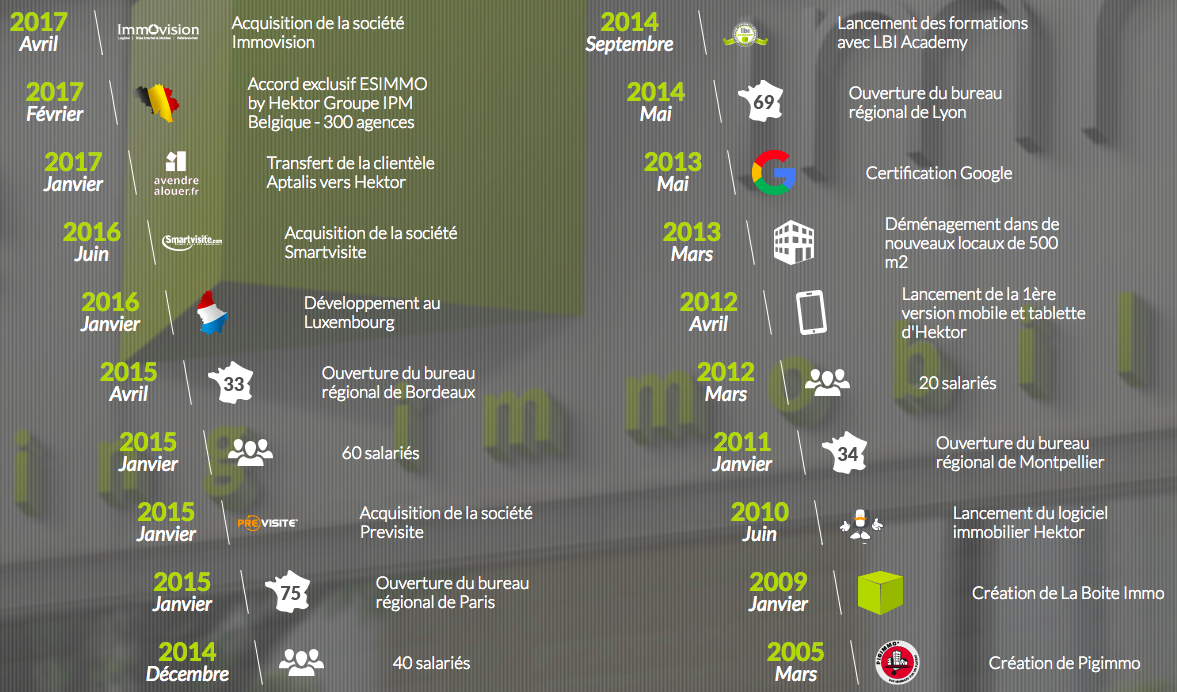
\includegraphics[width = 15cm]{historique.png}
        \textit{Historique graphique}
    \end{center} 

\chapter{Edouard}
    \begin{center}
    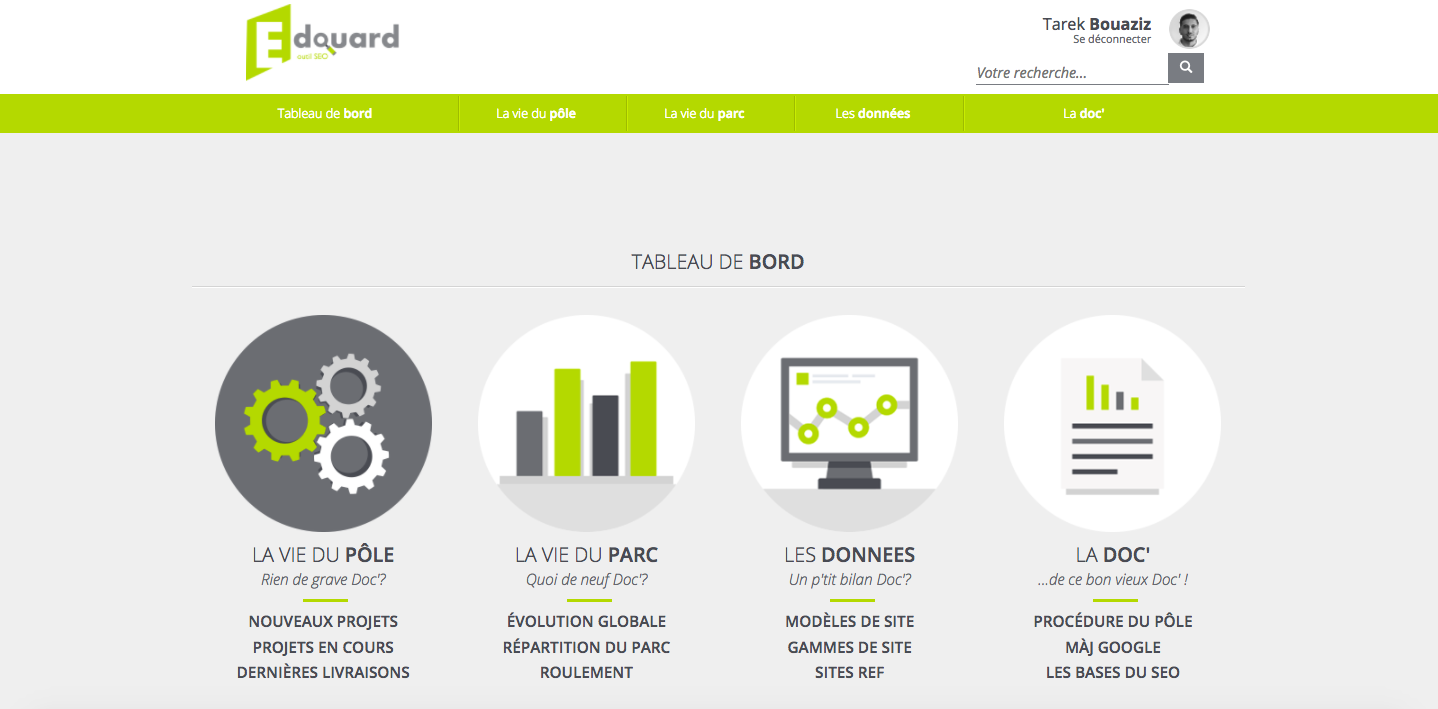
\includegraphics[width = 15cm]{accueilEdouard.png}
    \textit{Visuel de l'accueil de l'outil Edouard}
    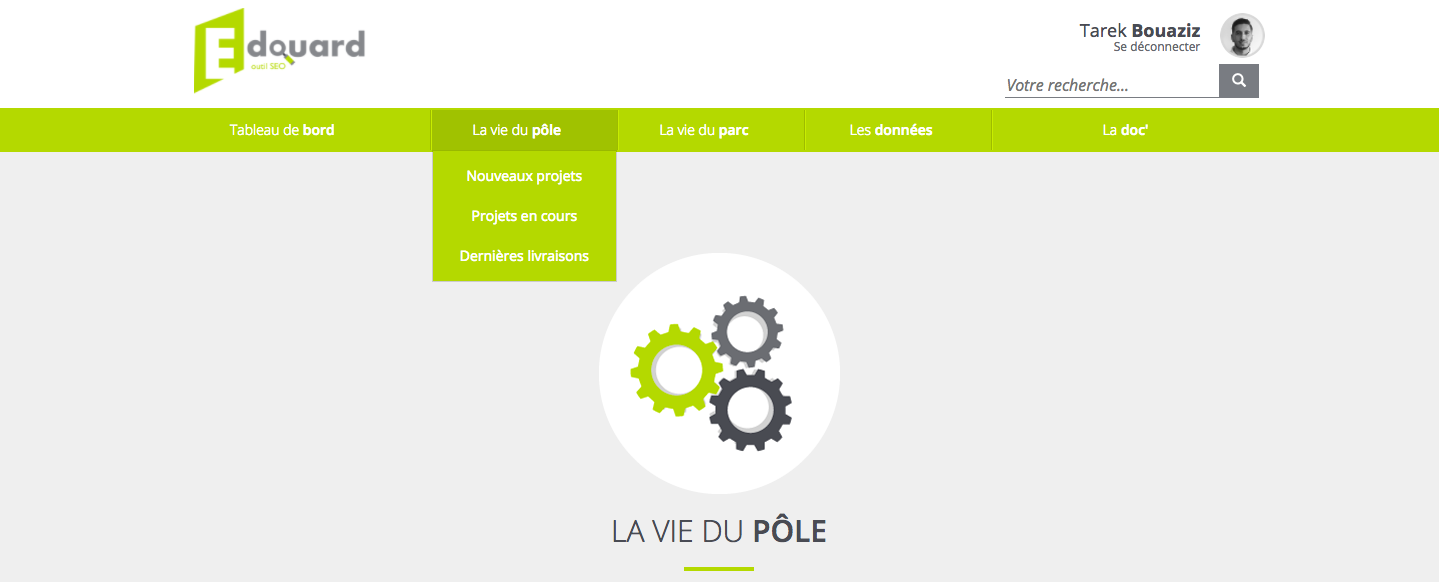
\includegraphics[width = 15cm]{viePole.png}
    \textit{Menu La Vie du Pôle}
    
    
\includegraphics[width = 15cm]{viePole2.png}
    \textit{Tableau de plannification}
    
    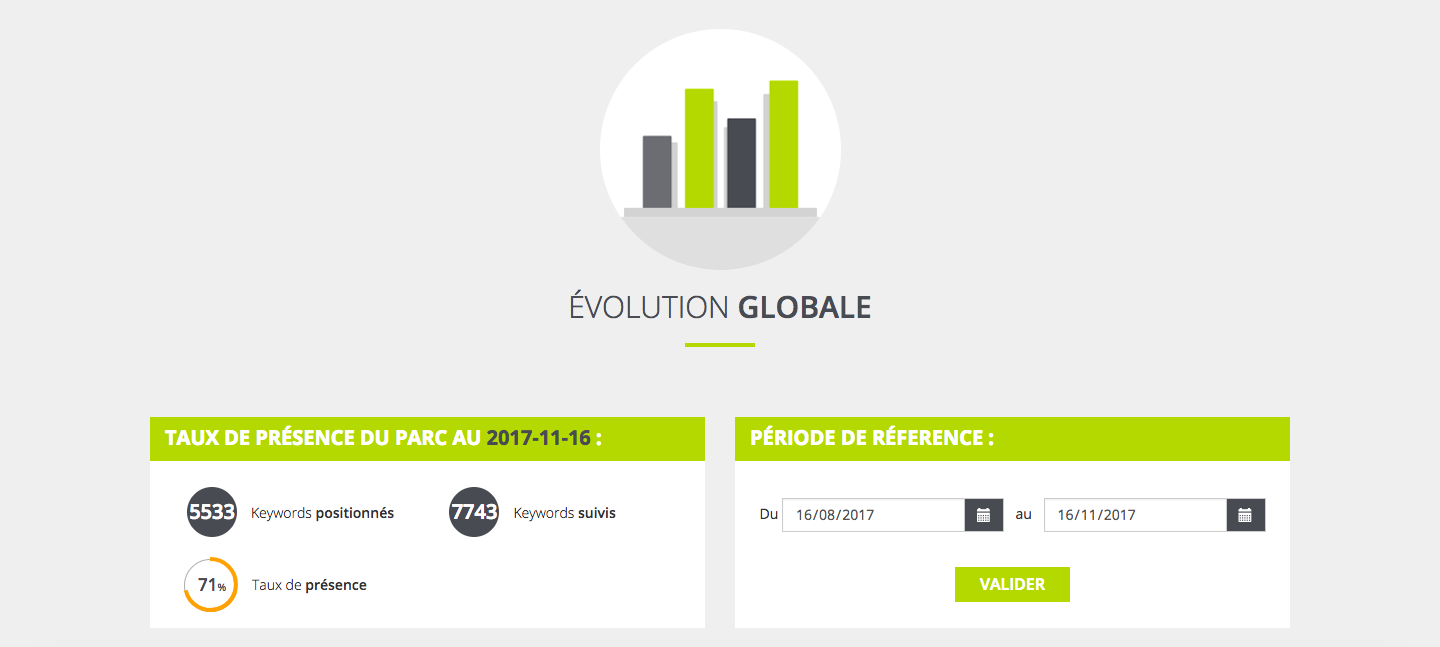
\includegraphics[width = 15cm]{vieParc.png}
    \textit{Page La Vie du Parc - Taux de présence et choix période}
    
    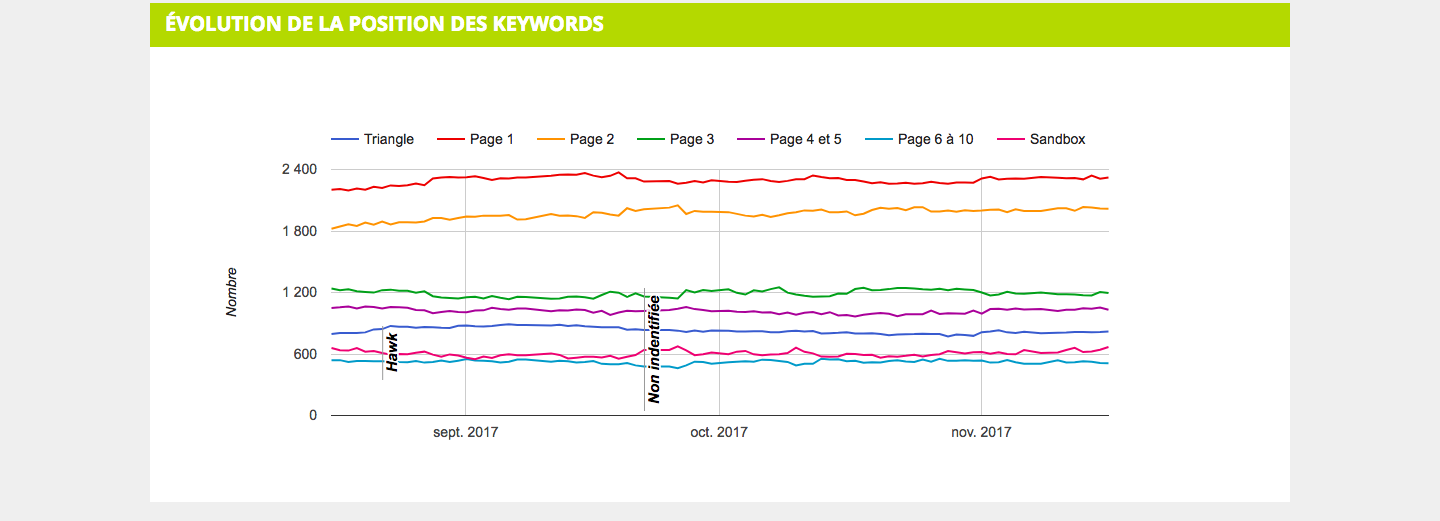
\includegraphics[width = 15cm]{vieParc2.png}
    \textit{Page La Vie du Parc - Evolution Globale}
    
    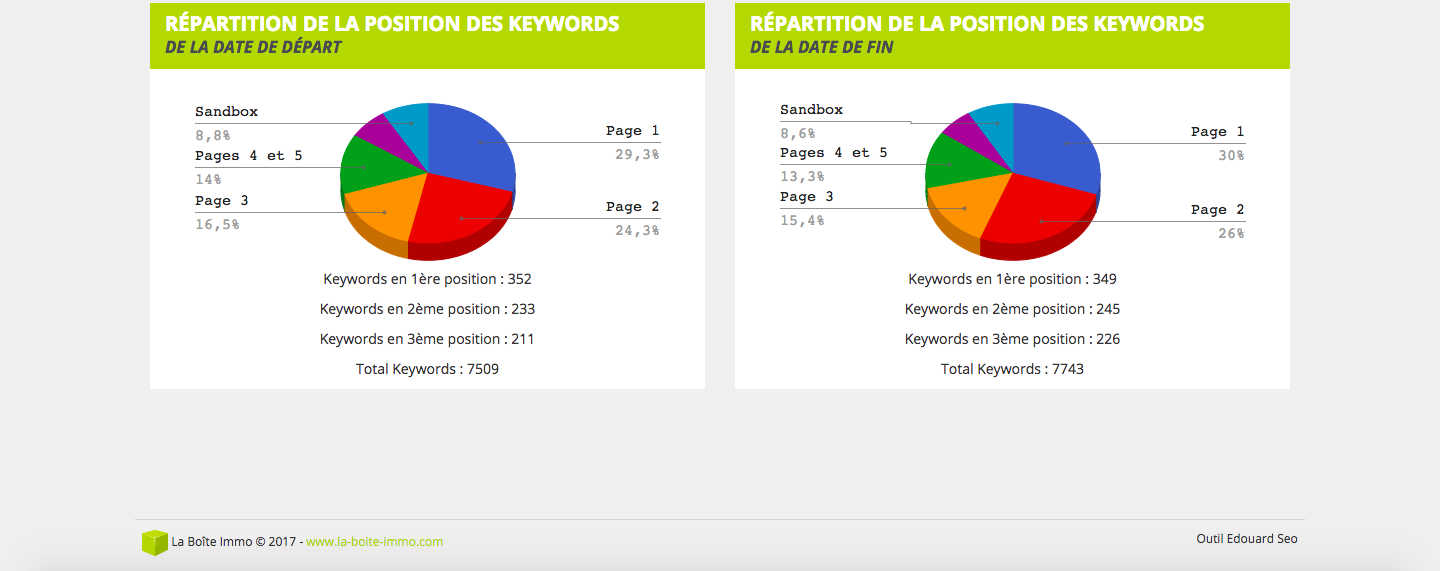
\includegraphics[width = 15cm]{vieParc3.png}
    \textit{Page La Vie du Parc - Répartition}
    
    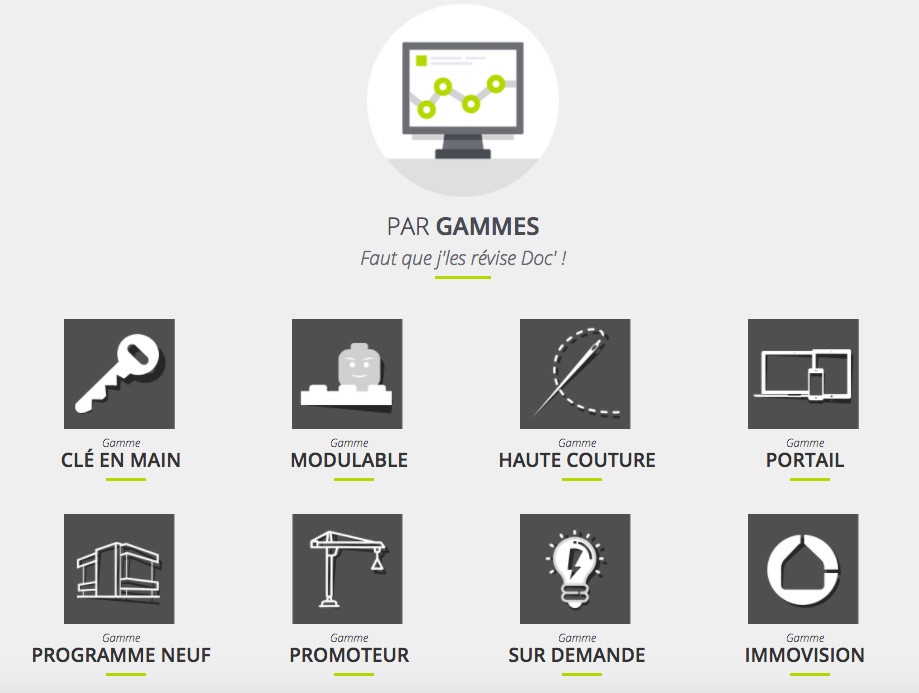
\includegraphics[width = 15cm]{dataModel.png}
    \textit{Page Les données - Données par gammes}
    
    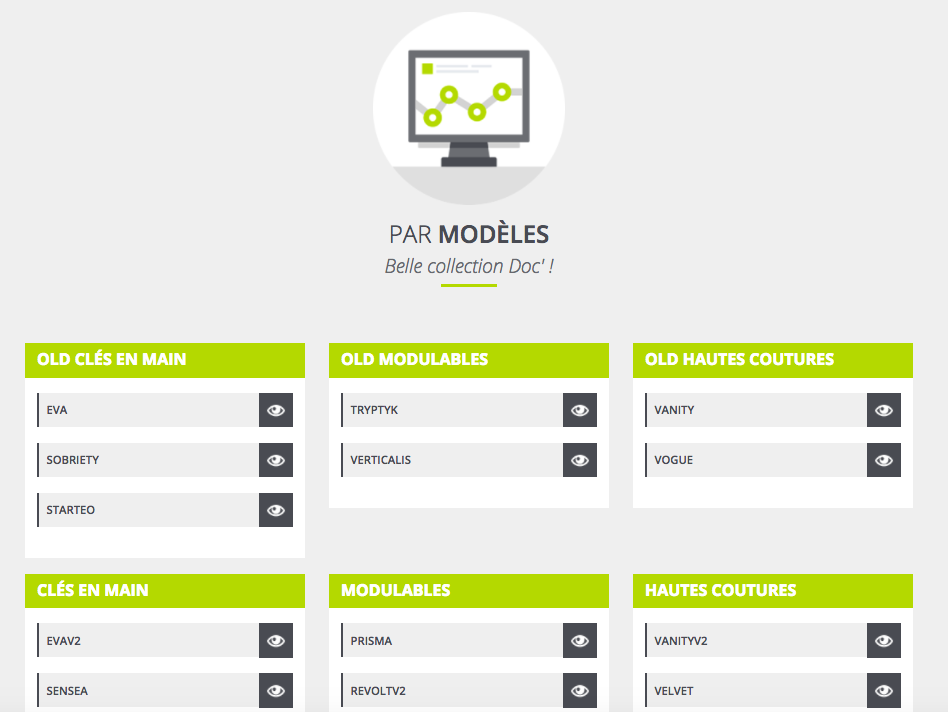
\includegraphics[width = 15cm]{modelData.png}
    \textit{Page Les données - Données par modèles}
    
    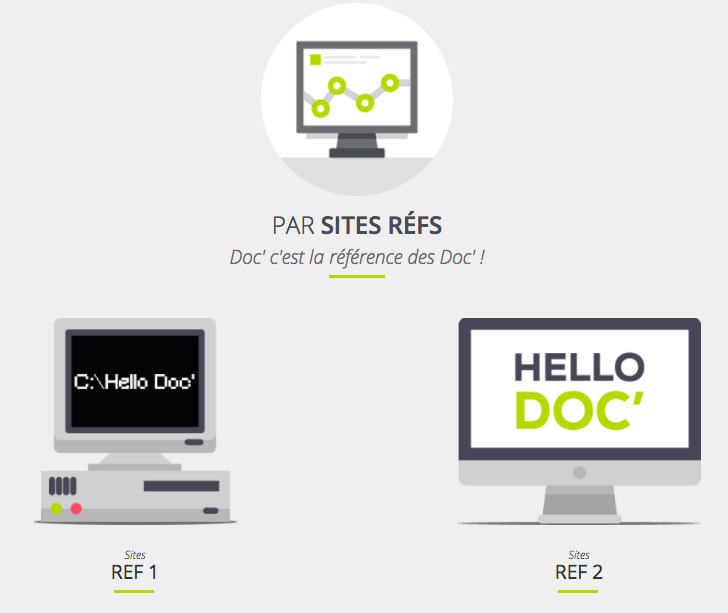
\includegraphics[width = 15cm]{siteRefData.png}
    \textit{Page Les données - Données par sites ref}
    
    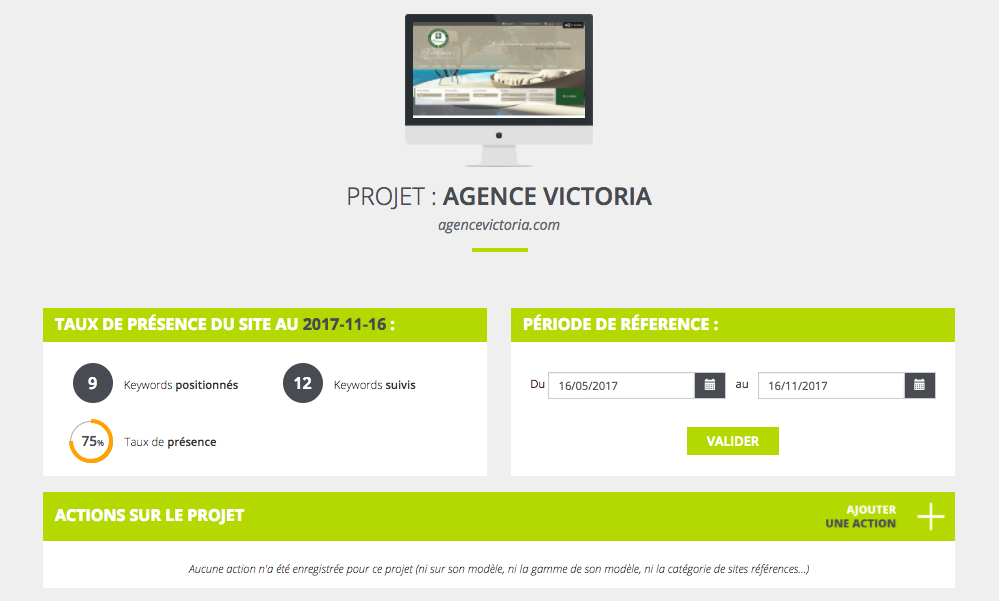
\includegraphics[width = 15cm]{projetData.png}
    \textit{Page Projet - Données par projet}
    
    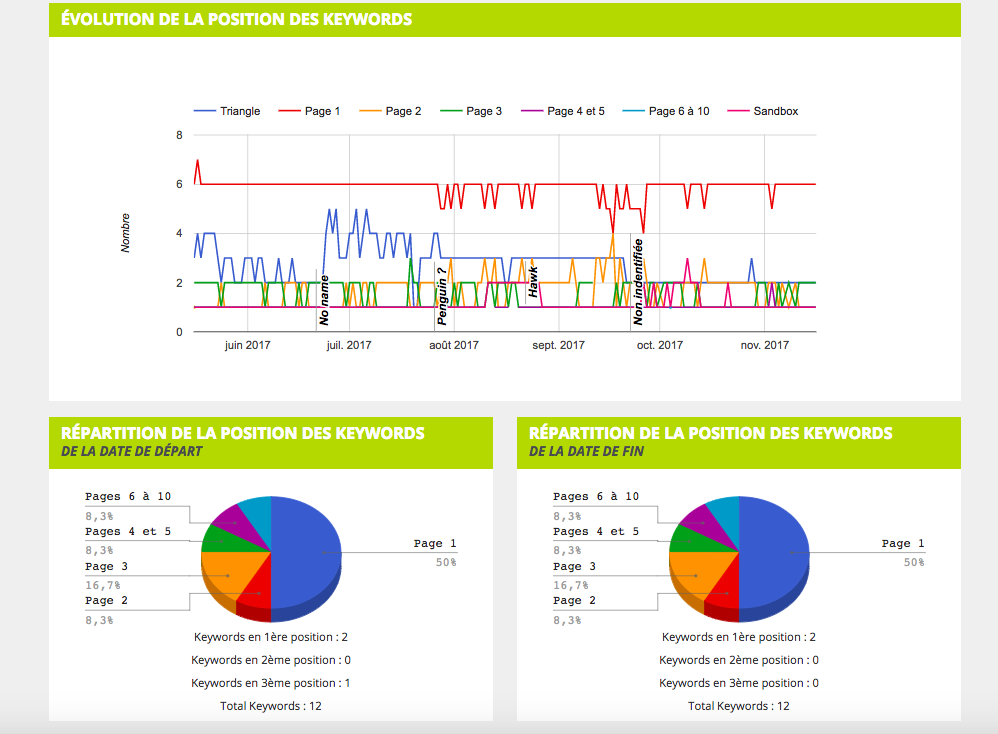
\includegraphics[width = 15cm]{projetData2.png}
    \textit{Page Projet - Evolution et répartitions des positions des mots clés}
    
    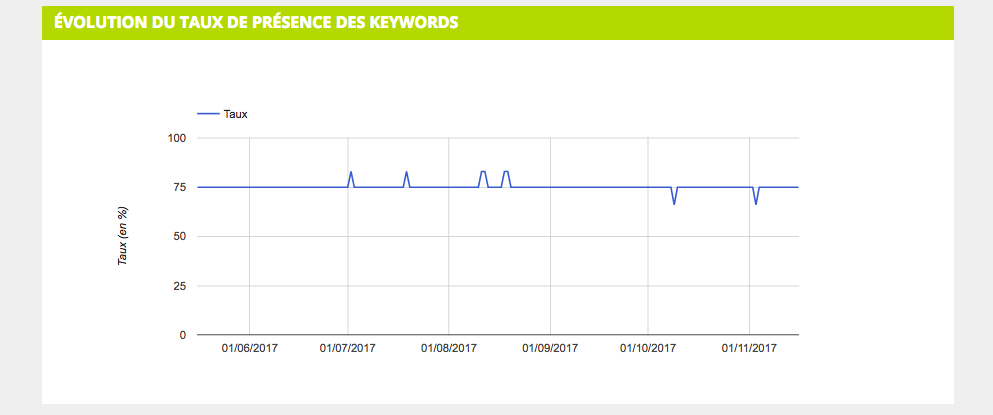
\includegraphics[width = 15cm]{projetData3.png}
    \textit{Page Projet - Evolution taux de présence}
    
    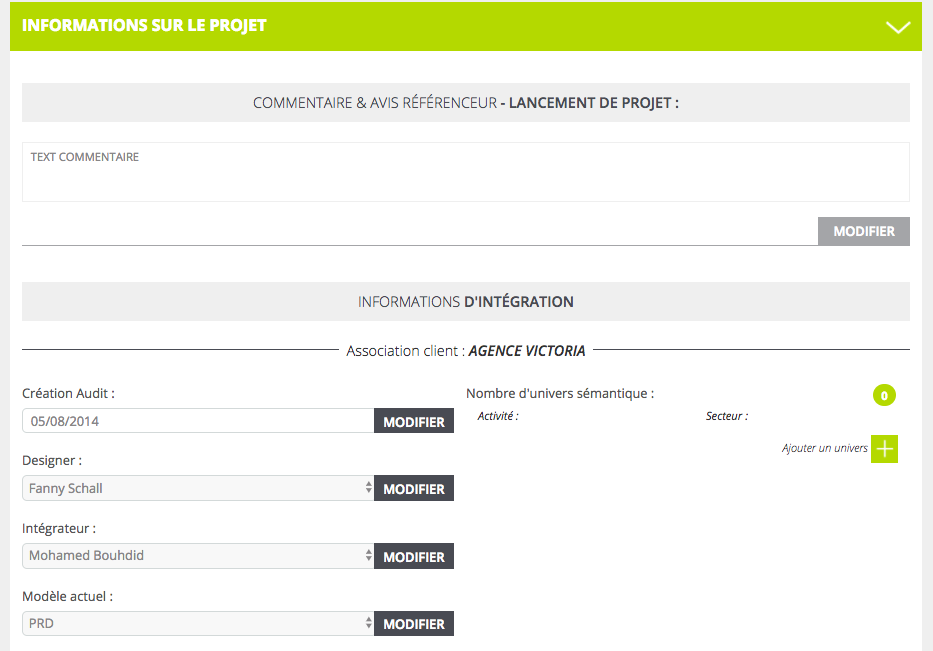
\includegraphics[width = 15cm]{projetData4.png}
    \textit{Page Projet - Informations sur le projet 1}
    
    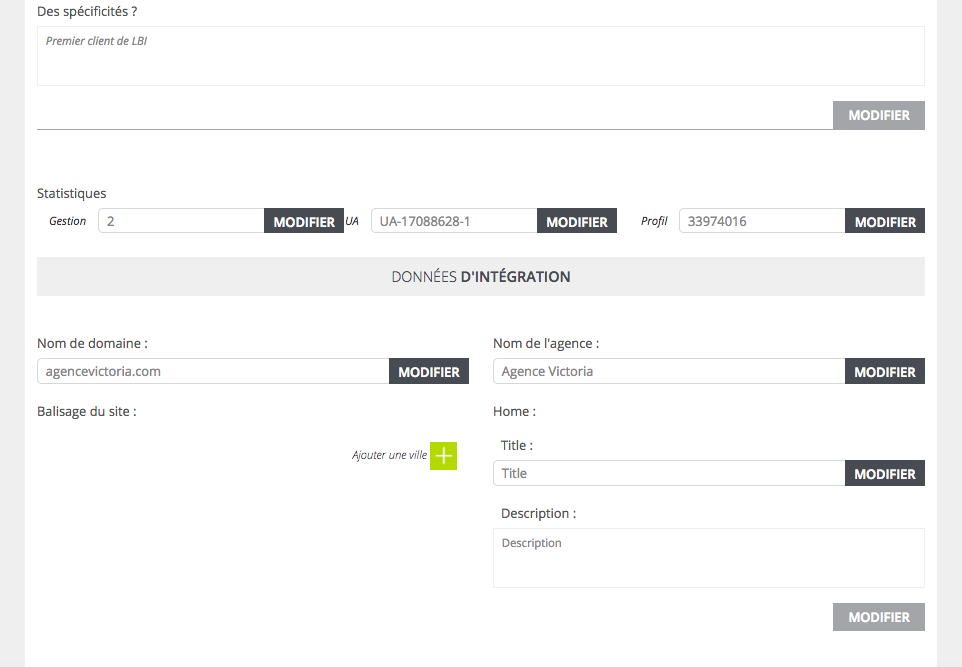
\includegraphics[width = 15cm]{projetData5.png}
    \textit{Page Projet - Informations sur le projet 2}
    
    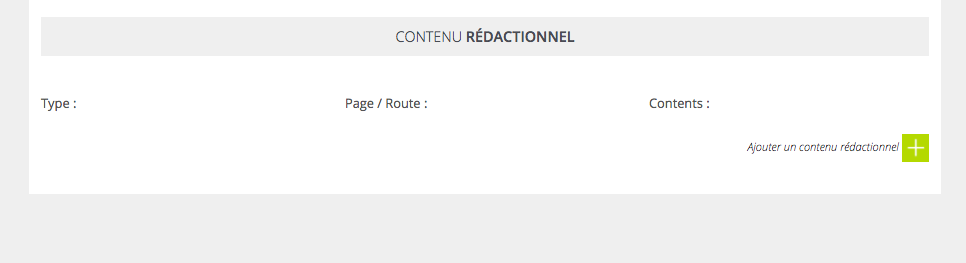
\includegraphics[width = 15cm]{projetData6.png}
    \textit{Page Projet - Informations sur le projet 3}
    
    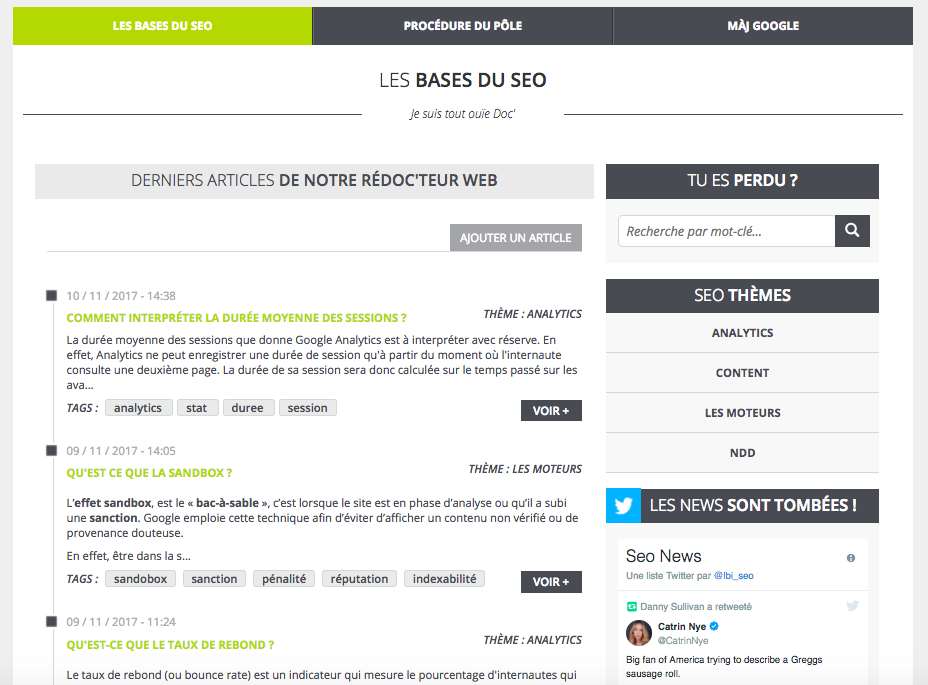
\includegraphics[width = 15cm]{blog.png}
    \textit{Page La Doc - Blog}
    \end{center} 
\end{appendix}

\end{document}